\documentclass[twoside, final]{hcmut_report}

% Packages for TikZ drawing
\usepackage{tikz}
\usepackage{circuitikz} % For electrical circuits
\usepackage{float}
\usepackage{enumitem}
\usepackage[T1]{fontenc}
\usetikzlibrary{shapes.geometric, arrows, positioning, patterns, decorations.pathmorphing}
\usepackage{booktabs}
\usepackage{multirow}
\usepackage{array}

% Configuration
\newcommand{\var}[1]{\textbf{#1}}
\DeclareRobustCommand{\code}[1]{\begingroup\def\_{\textunderscore\allowbreak}\textsf{#1}\endgroup}
\renewcommand{\texttt}[1]{\code{#1}}
\setlist[itemize]{leftmargin=2.2em,label=--,labelsep=0.6em,itemsep=0.35em,topsep=0.35em,parsep=0pt,partopsep=0pt,align=left}
\upperuniname{VIETNAM NATIONAL UNIVERSITY HO CHI MINH CITY}
\uniname{HO CHI MINH CITY UNIVERSITY OF TECHNOLOGY}
\deptname{FACULTY OF COMPUTER SCIENCE AND ENGINEERING}

\coursename{\LARGE Logic Design \\ \large (CO3097)}
\reporttype{\Large Report Lab 2}
\title{\Large SPI Protocol Module}

\advisor{
Ton Huynh Long
}
\student{
   Nguyen Chi Thanh, 2313078
   Nguyen Viet Hoang, 2311066
   Le Duc Tai, 2312995
   Mai Xuan Nhut, 2312549
}
\setlength{\parindent}{2em}
\begin{document}
\coverpage
\pagestyle{empty}
\tableofcontents
\pagestyle{fancy}
\pagebreak

\section{Interface}
\subsection{Top-Level Module Interface (\texttt{Cubic\_Solver})}
The \texttt{Cubic\_Solver} module acts as the system wrapper. It accepts four FP32 coefficients representing the cubic equation $ax^3 + bx^2 + cx + d = 0$ and computes up to three complex roots formatted in coordinate form ($x\_re + j \cdot x\_im$). The control flow is governed by a standard handshake mechanism consisting of \texttt{start} and \texttt{done} signals.

\begin{figure}[H]
    \centering
    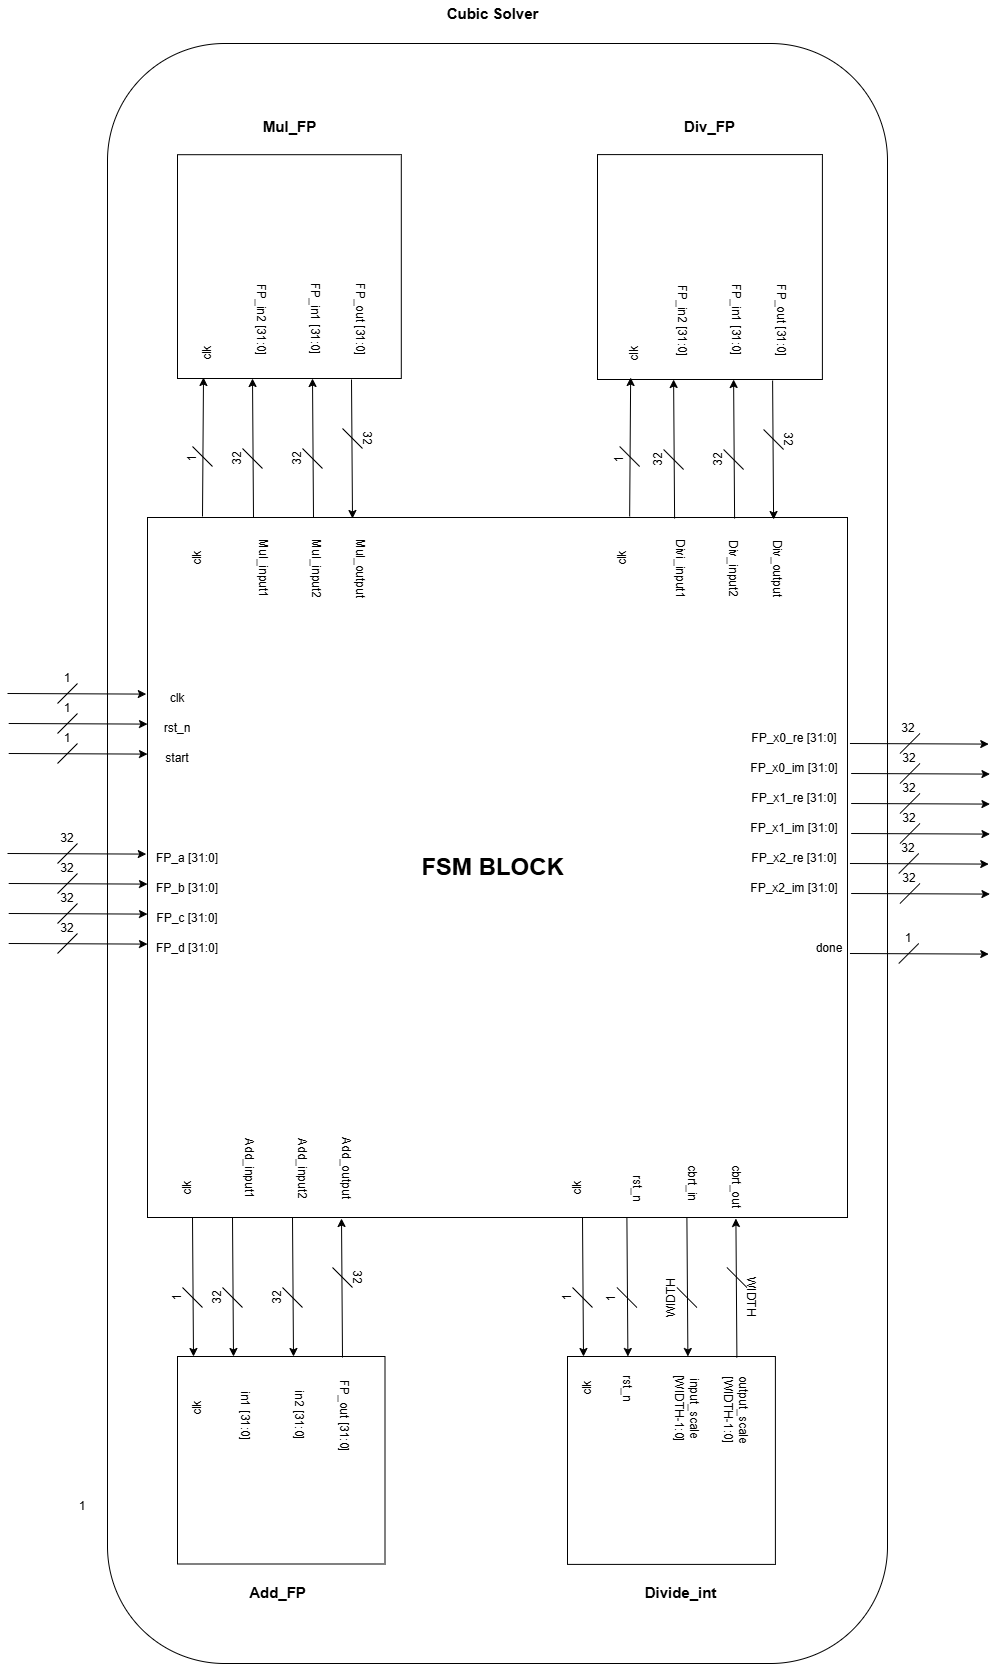
\includegraphics[width=0.6\textwidth]{graphics/cubic_solver.png}
    \caption{Top-Level Block Diagram and Interface of the Cubic Solver Module}
    \label{fig:cubic_solver_interface}
\end{figure}

The physical and logical boundary of this top-level module is defined by the following signaling groups:
\begin{itemize}
    \item [\texttt{clk} (Input, 1-bit):] Global system clock, driving all internal finite state machines (FSM) and pipeline registers on its positive edge.
    \item [\texttt{rst\_n} (Input, 1-bit):] Active-low asynchronous reset, forcing the control logic back to the \texttt{IDLE} state and clearing intermediate data registers.
    \item[\texttt{start} (Input, 1-bit):] Synchronous control pulse that triggers the FSM execution sequence. Must be asserted for at least one clock cycle to latch the input coefficients.
    \item[\texttt{FP\_a, FP\_b, FP\_c, FP\_d} (Inputs, 32-bit Bus):] Single-precision floating-point ports assigned to input the cubic equation coefficients $a, b, c,$ and $d$ respectively.
    \item[\texttt{done} (Output, 1-bit):] Handshake termination flag. Asserted high for exactly one clock cycle when the final root calculation stage is complete and valid data is locked on the outputs.
    \item[\texttt{FP\_x0\_re, FP\_x1\_re, FP\_x2\_re} (Outputs, 32-bit Bus):] Ports dedicated to outputting the real parts ($\text{Real}[x_n]$) of the three calculated roots in standard IEEE 754 single-precision format.
    \item[\texttt{FP\_x0\_im, FP\_x1\_im, FP\_x2\_im} (Outputs, 32-bit Bus):] Ports dedicated to outputting the imaginary parts ($\text{Imag}[x_n]$) of the three roots. For purely real roots, these outputs drive a static $32'h0000\_0000$ vector.
\end{itemize}

\subsection{Signed Integer Divider Interface (\texttt{Divide\_int})}
The \texttt{Divide\_int} module is a dedicated arithmetic component designed to handle signed 8-bit integer division. Within the \texttt{Cubic\_Solver} architecture, this module is specifically utilized to scale the exponents of floating-point numbers during the cube root calculation phase ($cbrt$). It operates purely on signed exponents to determine the proper scaling factor before normalization.

\begin{figure}[H]
    \centering
    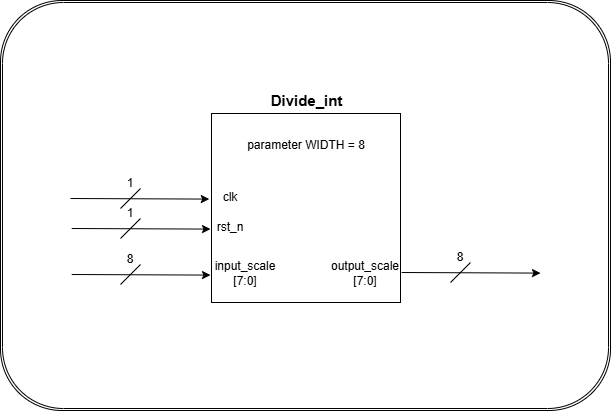
\includegraphics[width=0.5\textwidth]{graphics/div_int.png}
    \caption{Port Interface of the Signed Integer Exponent Divider Module}
    \label{fig:divide_int_interface}
\end{figure}

The hardware boundary of this helper block is defined as a purely arithmetic combinational module with the following ports:
\begin{itemize}
    \item[\texttt{input\_scale} (Input, 8-bit Bus):] Two's complement signed 8-bit integer vector carrying the raw, unadjusted exponent bias derived from the intermediate radical components.
    \item[\texttt{output\_scale} (Output, 8-bit Bus):] Two's complement signed 8-bit integer vector containing the mathematically scaled quotient value, passed directly back to the exponent adjustment logic of the cube-root normalization step.
\end{itemize}

\subsection{Floating-Point Divider Interface (\texttt{Div\_FP})}
The \texttt{Div\_FP} module implements a 16-cycle pipelined division using a Radix-4 algorithm. It comprises an input register stage, 14 iterative pipeline stages generating 2 quotient bits per cycle, and a final rounding and packing combinational unit.

\begin{figure}[H]
    \centering
    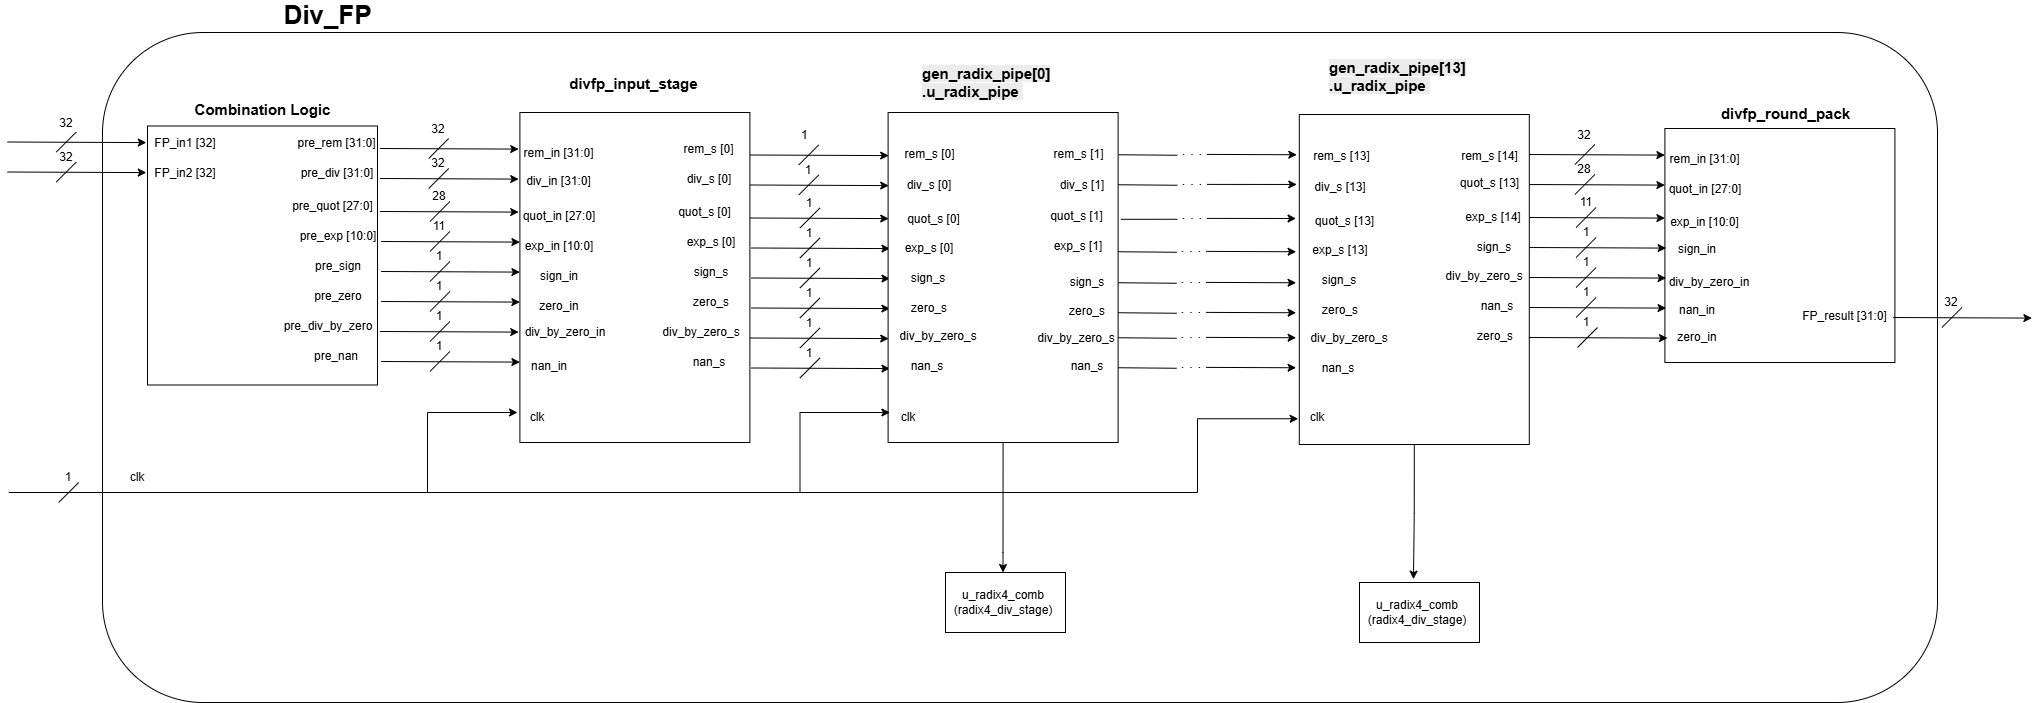
\includegraphics[width=0.9\textwidth]{graphics/div_FP.png}
    \caption{Internal Pipeline Architecture and Port Interfaces of \texttt{Div\_FP}}
    \label{fig:div_fp_interface}
\end{figure}

The macro signaling interface of the division datapath interacts via the following dedicated terminals:
\begin{itemize}
    \item[\texttt{clk} (Input, 1-bit):] Dedicated clock input running synchronously with the main system clock to toggle the 14 internal pipeline stage barriers (\texttt{gen\_radix\_pipe[0]} through \texttt{[13]}).
    \item[\texttt{FP\_in1} (Input, 32-bit Bus):] Single-precision floating-point input representing the dividend ($A$) vector.
    \item[\texttt{FP\_in2} (Input, 32-bit Bus):] Single-precision floating-point input representing the divisor ($B$) vector.
    \item[\texttt{FP\_out} (Output, 32-bit Bus):] Pipelined output port that delivers the stabilized, normalized, and rounded single-precision quotient result vector ($A/B$) after a deterministic execution latency of 16 clock cycles.
\end{itemize}

\subsection{Floating-Point Multiplier Interface (\texttt{Mul\_FP})}
The \texttt{Mul\_FP} module performs single-precision multiplication using a multi-stage architecture. It encapsulates the \texttt{MFP\_Mul} core module, which hosts a 6-stage partial product accumulation pipeline utilizing \texttt{Mul24x4} arithmetic array sub-blocks, and the \texttt{MFP\_Norm\_Rounding} unit for normalization.

\subsubsection{Module-Level External Interface}
This sub-section defines the top-level boundary of the \texttt{Mul\_FP} module. It handles the external handshaking and the raw FP32 data vectors before passing them to the internal execution cores.

\begin{figure}[H]
    \centering
    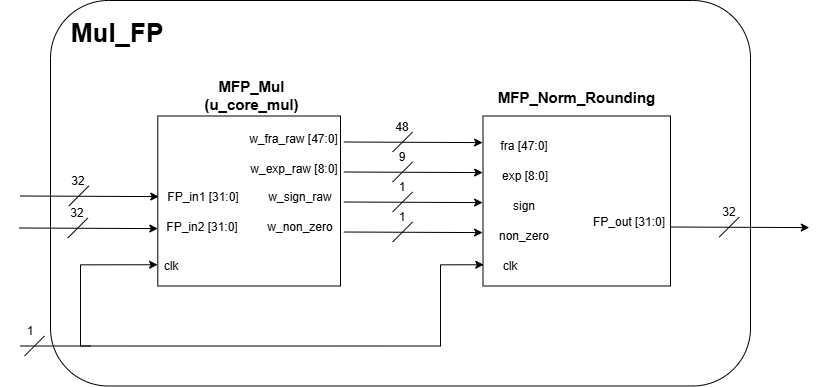
\includegraphics[width=0.7\textwidth]{graphics/mul_FP.png}
    \caption{Detailed Datapath and Port Interconnections of the Pipelined Multiplier \texttt{Mul\_FP}}
    \label{fig:mul_fp_interface}
\end{figure}

The physical external wrapper of the multi-cycle multiplier consists of the following standard ports:
\begin{itemize}
    \item[\texttt{clk} (Input, 1-bit):] Main clock connection used to advance the hidden pipeline arrays inside both the multiplication matrix and the output rounding register stage.
    \item[\texttt{FP\_in1} (Input, 32-bit Bus):] FP32 multiplicand operand input vector ($A$).
    \item[\texttt{FP\_in2} (Input, 32-bit Bus):] FP32 multiplier operand input vector ($B$).
    \item[\texttt{FP\_out} (Output, 32-bit Bus):] Standardized 32-bit IEEE 754 product result vector ($A \times B$) exposed to the central system bus.
\end{itemize}

\subsubsection{Internal Partial Product Shift-and-Add Interface}
Within the \texttt{MFP\_Mul} core, the intermediate accumulation stages (\texttt{Stage 1} through \texttt{Stage 5}) implement a hardware-optimized shift-and-add architecture. Instead of shifting the newly generated 28-bit partial product ($prod[i]$) to the left, the design shifts the previously accumulated sum ($buf\_stage_{i}$) to the right by 4 bits before feeding it into a dedicated fixed-point adder. The lower 4 bits of the old accumulator bypass the adder entirely and are directly concatenated back to form the updated bit-extended product, significantly minimizing critical path delay and saving hardware routing resources.

\begin{figure}[H]
    \centering
    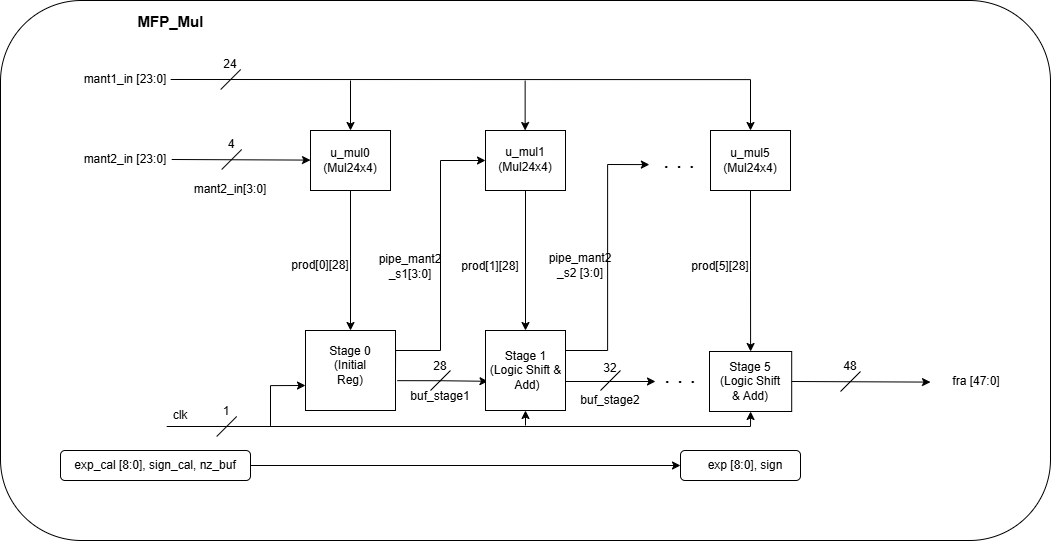
\includegraphics[width=0.8\textwidth]{graphics/MFP_mul_core.png}
    \caption{Detailed Internal Datapath of the Shift-and-Add Mechanism inside Pipeline Stages}
    \label{fig:shift_and_add_logic}
\end{figure}

The data interaction traversing the sub-boundaries of the sequential pipeline stages is formalized as follows:
\begin{itemize}
    \item[\texttt{prod[i]} (Internal Input, 28-bit Bus):] The localized static 28-bit product coming from the combinatorial \texttt{Mul24x4} array block, computed by multiplying the full 24-bit mantissa of operand $A$ with a specific 4-bit slice of operand $B$'s mantissa.
    \item[\texttt{buf\_stage\_in} (Internal Input, Variable Width):] The accumulated product bus received from the preceding stage's output register. This bus grows incrementally by 4 bits at each stage step (starting from 28 bits at \texttt{Stage 0} up to 44 bits when entering \texttt{Stage 5}).
    \item[\texttt{pipe\_mant2\_in} (Internal Input, Variable Width):] The unconsumed, remaining higher-order bits of operand $B$'s mantissa vector, shrinking by 4 bits per clock cycle as it slides through the pipeline.
    \item[\texttt{buf\_stage\_out} (Internal Output, Variable Width):] The newly calculated, bit-extended product sum captured by the localized stage register on the rising edge of the clock.
    \item[\texttt{pipe\_mant2\_out} (Internal Output, Variable Width):] The truncated multiplier $B$ vector, shifted right by 4 bits to prepare the next localized 4-bit nibble for the subsequent stage's arithmetic block.
\end{itemize}

\subsubsection{Normalization and Rounding Interface (\texttt{MFP\_Norm\_Rounding})}
After the 6-stage accumulation pipeline generates the raw 48-bit product, the datapath invokes the \texttt{MFP\_Norm\_Rounding} module. This final stage is responsible for adjusting the temporary exponent based on overflow detection, rounding the mantissa to fit the standard 23-bit width, and checking boundaries for underflow or overflow conditions.

\begin{figure}[H]
    \centering
    \includegraphics[width=0.65\textwidth]{graphics/MFP_norm_rounding.png}
    \caption{Detailed Internal Datapath of the Normalization and Rounding Mechanism}
    \label{fig:norm_rounding_logic}
\end{figure}

The sub-module interface of this normalization engine processes the following local connections:
\begin{itemize}
    \item[\texttt{w\_fra\_raw} (Internal Input, 48-bit Bus):] The final un-normalized, raw 48-bit product vector originating from the output registers of \texttt{Stage 5}.
    \item[\texttt{w\_exp\_raw} (Internal Input, 9-bit Bus):] The 9-bit unadjusted exponent sum vector calculated concurrently via the localized add operation ($E_a + E_b - 127$).
    \item[\texttt{w\_sign\_raw} (Internal Input, 1-bit):] The product parity flag bit derived from the structural asynchronous operation $S_a \oplus S_b$.
    \item[\texttt{w\_non\_zero} (Internal Input, 1-bit):] A structural zero-bypass status bit indicating whether the incoming floating-point operands are nonzero values.
\end{itemize}

\subsection{Floating-Point Adder/Subtractor Interface (\texttt{Add\_FP})}
The \texttt{Add\_FP} core executes floating-point addition and subtraction wrapped inside a 5-stage pipeline macro. The internal datapath splits the processing into sequential steps: exponent comparison (\texttt{u\_stage1}), mantissa alignment shifting (\texttt{u\_stage2}), fixed-point additions (\texttt{u\_stage3}), leading-one normalization detection (\texttt{u\_stage4}), and post-computation rounding (\texttt{u\_stage5}).

\begin{figure}[H]
    \centering
    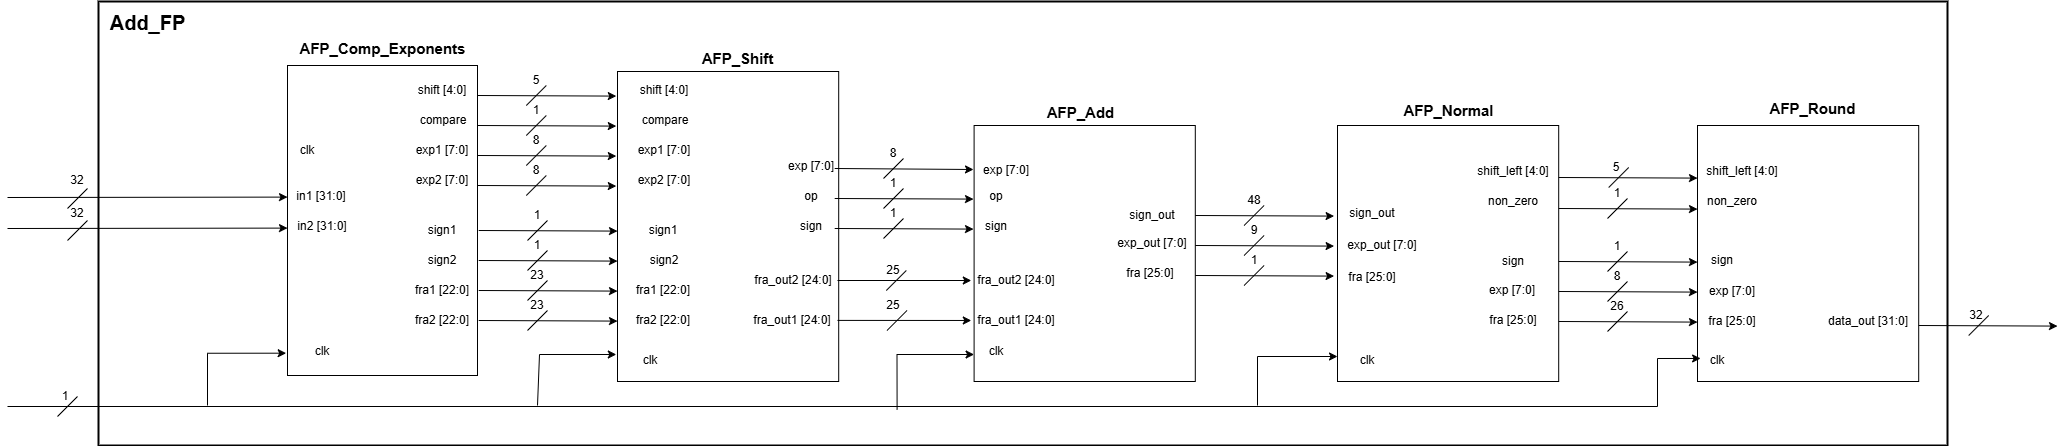
\includegraphics[width=0.7\textwidth]{graphics/add_FP.png}
    \caption{Structural Sub-module Interconnections and Interface of \texttt{Add\_FP}}
    \label{fig:add_fp_interface}
\end{figure}

The I/O interface pins bound to this algebraic calculation core are specified below:
\begin{itemize}
    \item[\texttt{clk} (Input, 1-bit):] Main clock line driving the synchronous state boundaries of the 5 internal pipeline processing blocks (\texttt{u\_stage1} through \texttt{u\_stage5}).
    \item[\texttt{in1} (Input, 32-bit Bus):] FP32 vector acting as the augend during addition operations or the minuend during subtraction operations.
    \item[\texttt{in2} (Input, 32-bit Bus):] FP32 vector acting as the addend during addition operations or the subtrahend during subtraction operations.
    \item[\texttt{data\_out} (Output, 32-bit Bus):] Stabilized 32-bit IEEE 754 single-precision sum or difference result vector, available exactly 5 clock cycles after the corresponding operands are loaded into the first stage.
\end{itemize}
% \include{contents/FSM}
% \section{Functional implementation}

\subsection{Floating-point arithmetic subsystem}

The arithmetic subsystem is the computational backbone of the solver. The design philosophy is to build one reusable IEEE-754 FP32 arithmetic library, then let the top-level controller schedule these blocks repeatedly to evaluate the cubic-solving algorithm. In other words, the project follows a \textbf{shared datapath + control FSM} strategy instead of instantiating a separate arithmetic network for each formula. This approach has three advantages:
\begin{itemize}[noitemsep]
    \item it keeps the architecture structurally regular and easier to debug
    \item it allows the same arithmetic blocks to be reused in coefficient normalization, discriminant computation, iterative approximation, and final root reconstruction
    \item it makes the behavior of the hardware closely match the golden model, where each high-level formula is also decomposed into a sequence of primitive operations
\end{itemize}

\subsubsection{Adder module}
The \texttt{Add\_FP} module performs both addition and subtraction on FP32 operands.
\begin{itemize}[noitemsep]
    \item \textbf{Operand alignment}: the exponents are compared first so that the smaller mantissa can be right-shifted before accumulation.
    \item \textbf{Unified add/sub datapath}: subtraction is implemented implicitly by changing operand signs and by using the internal \texttt{op} control signal.
    \item \textbf{Normalization and rounding}: after mantissa accumulation, the result is normalized and packed back into IEEE-754 format.
\end{itemize}

\subsubsection{Multiplier module}
The \texttt{Mul\_FP} module computes the product of two FP32 numbers through a pipelined mantissa multiplier followed by normalization and rounding.
\begin{itemize}[noitemsep]
    \item \textbf{Sign and exponent processing}: the output sign is obtained by XOR, while the output exponent is formed by exponent addition and bias correction.
    \item \textbf{Mantissa product generation}: the 24-bit mantissas are multiplied with a staged partial-product architecture.
    \item \textbf{High reuse}: the module is repeatedly used to evaluate powers, cross-products, and complex arithmetic terms during Pad\'e iterations.
\end{itemize}

\subsubsection{Divider module}
The \texttt{Div\_FP} module evaluates one FP32 division through a radix-4 pipelined divider.
\begin{itemize}[noitemsep]
    \item \textbf{Pre-processing}: sign, zero cases, division-by-zero, NaN, and exponent difference are identified before quotient generation.
    \item \textbf{Radix-4 quotient generation}: each stage emits two quotient bits, which provides a predictable latency suitable for controller scheduling.
    \item \textbf{Round-pack stage}: the quotient is converted back into a normalized IEEE-754 result before being registered at the output.
\end{itemize}

\subsection{Main solver behavior}

The \texttt{Cubic\_Solver} module is a controller-centric architecture. Its main responsibility is not to compute every formula in parallel, but to orchestrate the arithmetic modules so that the correct operands are presented to \texttt{Add\_FP}, \texttt{Mul\_FP}, and \texttt{Div\_FP} at the correct cycle offsets. Each state of the FSM corresponds to one algorithmic phase, while \texttt{delay\_count} acts as a micro-scheduler that determines which arithmetic expression is being issued in that phase.

Functionally, the top-level solver performs the following sequence:
\begin{enumerate}
    \item Capture input coefficients and standardize them by dividing with $-3a$.
    \item Compute $\Delta_0$, $\Delta_1$, and $\Delta$.
    \item Classify the equation into one of the three solution branches.
    \item Execute the square-root iteration for $\sqrt{\Delta}$ or $\sqrt{-\Delta}$.
    \item Execute the cube-root iteration in either real or complex mode to obtain $C$.
    \item Combine $\hat{b}$, $C$, $\overline{C}$, and $\Delta_0/C$ to generate the three final roots.
\end{enumerate}

At the implementation level, this sequence is realized by repeatedly reconfiguring the inputs of the three arithmetic blocks:
\begin{itemize}[noitemsep]
    \item \texttt{MulInput1/2} carry products such as $\hat{b}^2$, $\hat{b}^3$, $\Delta_1^2$, $P^2$, $P^3$, and the real/imaginary cross-products used in complex cube-root iteration.
    \item \texttt{AddInput1/2} combine intermediate terms into expressions such as $\Delta_0$, $\Delta_1$, $3S$, $3P^2+S$, $2P^3+S$, and the final root formulas.
    \item \texttt{DivInput1/2} are used whenever the algorithm requires normalization by division, Pad\'e update evaluation, or the quotient $\Delta_0/C$.
\end{itemize}

This means the top-level block is best interpreted as a scheduled arithmetic engine rather than a static combinational solver.

\subsection{Main control signals}

The most important control intent of the design is concentrated in a small set of scheduling and branch signals. Their functional roles are summarized in Table~\ref{tab:control_signals}.

\begin{table}[H]
\centering
\caption{Main control and scheduling signals in \texttt{Cubic\_Solver}}
\label{tab:control_signals}
\renewcommand{\arraystretch}{1.2}
\begin{tabular}{p{3.0cm} p{2.0cm} p{1.4cm} p{8.0cm}}
\toprule
\textbf{Signal} & \textbf{Type} & \textbf{Width} & \textbf{Functional meaning} \\
\midrule
\texttt{state} & Reg & 4 & Current state of the main finite state machine. Selects the active computational phase. \\
\texttt{next\_state} & Reg & 4 & Next-state combinational result derived from the current state, counters, and branch conditions. \\
\texttt{case\_index} & Reg & 2 & Encodes the selected solution branch: negative discriminant, simplified real branch, or general real branch. \\
\texttt{delay\_count} & Reg & 7 & Fine-grain schedule counter used to align operand issue with the latency of arithmetic pipelines. \\
\texttt{iteration\_count} & Reg & 5 & Counts the number of Pad\'e iterations already completed for square-root or cube-root evaluation. \\
\texttt{READY\_BRANCH\_CHECK} & Reg & 1 & Internal synchronization flag indicating that the branch-specific cube-root input and initial estimate are ready. \\
\texttt{MulInput1}, \texttt{MulInput2} & Reg & 32 each & Operands dispatched to the shared floating-point multiplier at the current cycle. \\
\texttt{AddInput1}, \texttt{AddInput2} & Reg & 32 each & Operands dispatched to the shared floating-point adder at the current cycle. \\
\texttt{DivInput1}, \texttt{DivInput2} & Reg & 32 each & Operands dispatched to the shared floating-point divider at the current cycle. \\
\texttt{cbrt\_scale\_in} & Reg & 8 & Exponent-related helper input used to construct the initial estimate for cube-root iteration. \\
\texttt{exponent\_max} & Reg & 8 & Stores the larger exponent between the real and imaginary parts when a complex cube-root seed is required. \\
\texttt{done} & Reg & 1 & Output completion flag asserted in the \texttt{DONE} state. \\
\bottomrule
\end{tabular}
\end{table}

\subsection{The internal registers}

Besides the explicit control signals, the solver uses a compact set of internal registers to hold operands and intermediate results between states:
\begin{itemize}[noitemsep]
    \item \texttt{r\_a}, \texttt{r\_b}, \texttt{r\_c}, \texttt{r\_d}: working coefficients. After the \texttt{STANDARDIZE} state, these registers no longer contain the original input values but the normalized coefficients used by the algorithm.
    \item \texttt{r\_delta\_0}, \texttt{r\_delta\_1}, \texttt{r\_delta}: algebraic invariants used for branch classification and final-root reconstruction.
    \item \texttt{r\_sqrt\_input}, \texttt{r\_sqrt\_output}: operand and current estimate for Pad\'e square-root iteration.
    \item \texttt{r\_cbrt\_re\_input}, \texttt{r\_cbrt\_im\_input}: real and imaginary parts of the cube-root operand.
    \item \texttt{r\_cbrt\_re\_output}, \texttt{r\_cbrt\_im\_output}: current cube-root estimate.
    \item \texttt{r\_C\_re}, \texttt{r\_C\_im}: final value of $C$ after the cube-root stage completes.
    \item \texttt{r\_temp[0:63]}: scratchpad register bank used to preserve pipeline results across multiple delay slots in long arithmetic schedules.
\end{itemize}

\subsection{Functional role of branch control and initialization}

The signal \texttt{case\_index} has a central functional meaning because it determines which numerical path the hardware will follow after the discriminant values have been computed:
\begin{itemize}[noitemsep]
    \item \texttt{2'b01}: discriminant is negative, so the solver must compute a complex-valued cube root and later generate roots from $C$ and $\overline{C}$.
    \item \texttt{2'b10}: special real branch with simplified cube-root evaluation.
    \item \texttt{2'b11}: general real branch, where the solver computes both $C$ and $\Delta_0/C$ before forming the three roots.
\end{itemize}
Because all later states depend on this 2-bit decision, the \texttt{CASE\_CHECK} and \texttt{BRANCH\_CHECK} states serve as the bridge between the algebraic invariants and the branch-specific datapath schedule.

Another important design feature is the use of \textbf{hardware-friendly initial estimates} for the iterative square-root and cube-root blocks.

For the square-root stage, the initial approximation is formed directly from the exponent field of the operand. The wire
\begin{equation}
\texttt{sqrt\_output\_exp = ((exp(\Delta) + 127) >> 1)}
\end{equation}
approximates the exponent of $\sqrt{\Delta}$, and the corresponding mantissa is copied to create \texttt{sqrt\_output\_init}. This gives the Pad\'e square-root iteration a starting point that is already close in magnitude to the true solution.

For the cube-root stage, the design uses the helper block \texttt{Divide\_int} to approximate the exponent transform
\begin{equation}
E_{\sqrt[3]{S}} \approx 127 + \frac{E_S - 127}{3}
\end{equation}
without invoking an additional floating-point divider. In the complex branch, the design first compares the exponents of the real and imaginary parts, selects the larger one as \texttt{exponent\_max}, and uses it to build a conservative initial estimate for the complex cube root. In the real branches, the exponent of the real operand alone is sufficient.

This initialization strategy is important because it reduces the number of Pad\'e iterations needed for convergence and makes the iterative states more stable in hardware.

\section{Internal implementation}

\subsection{Overall architecture}

\begin{figure}[H]
    \centering
    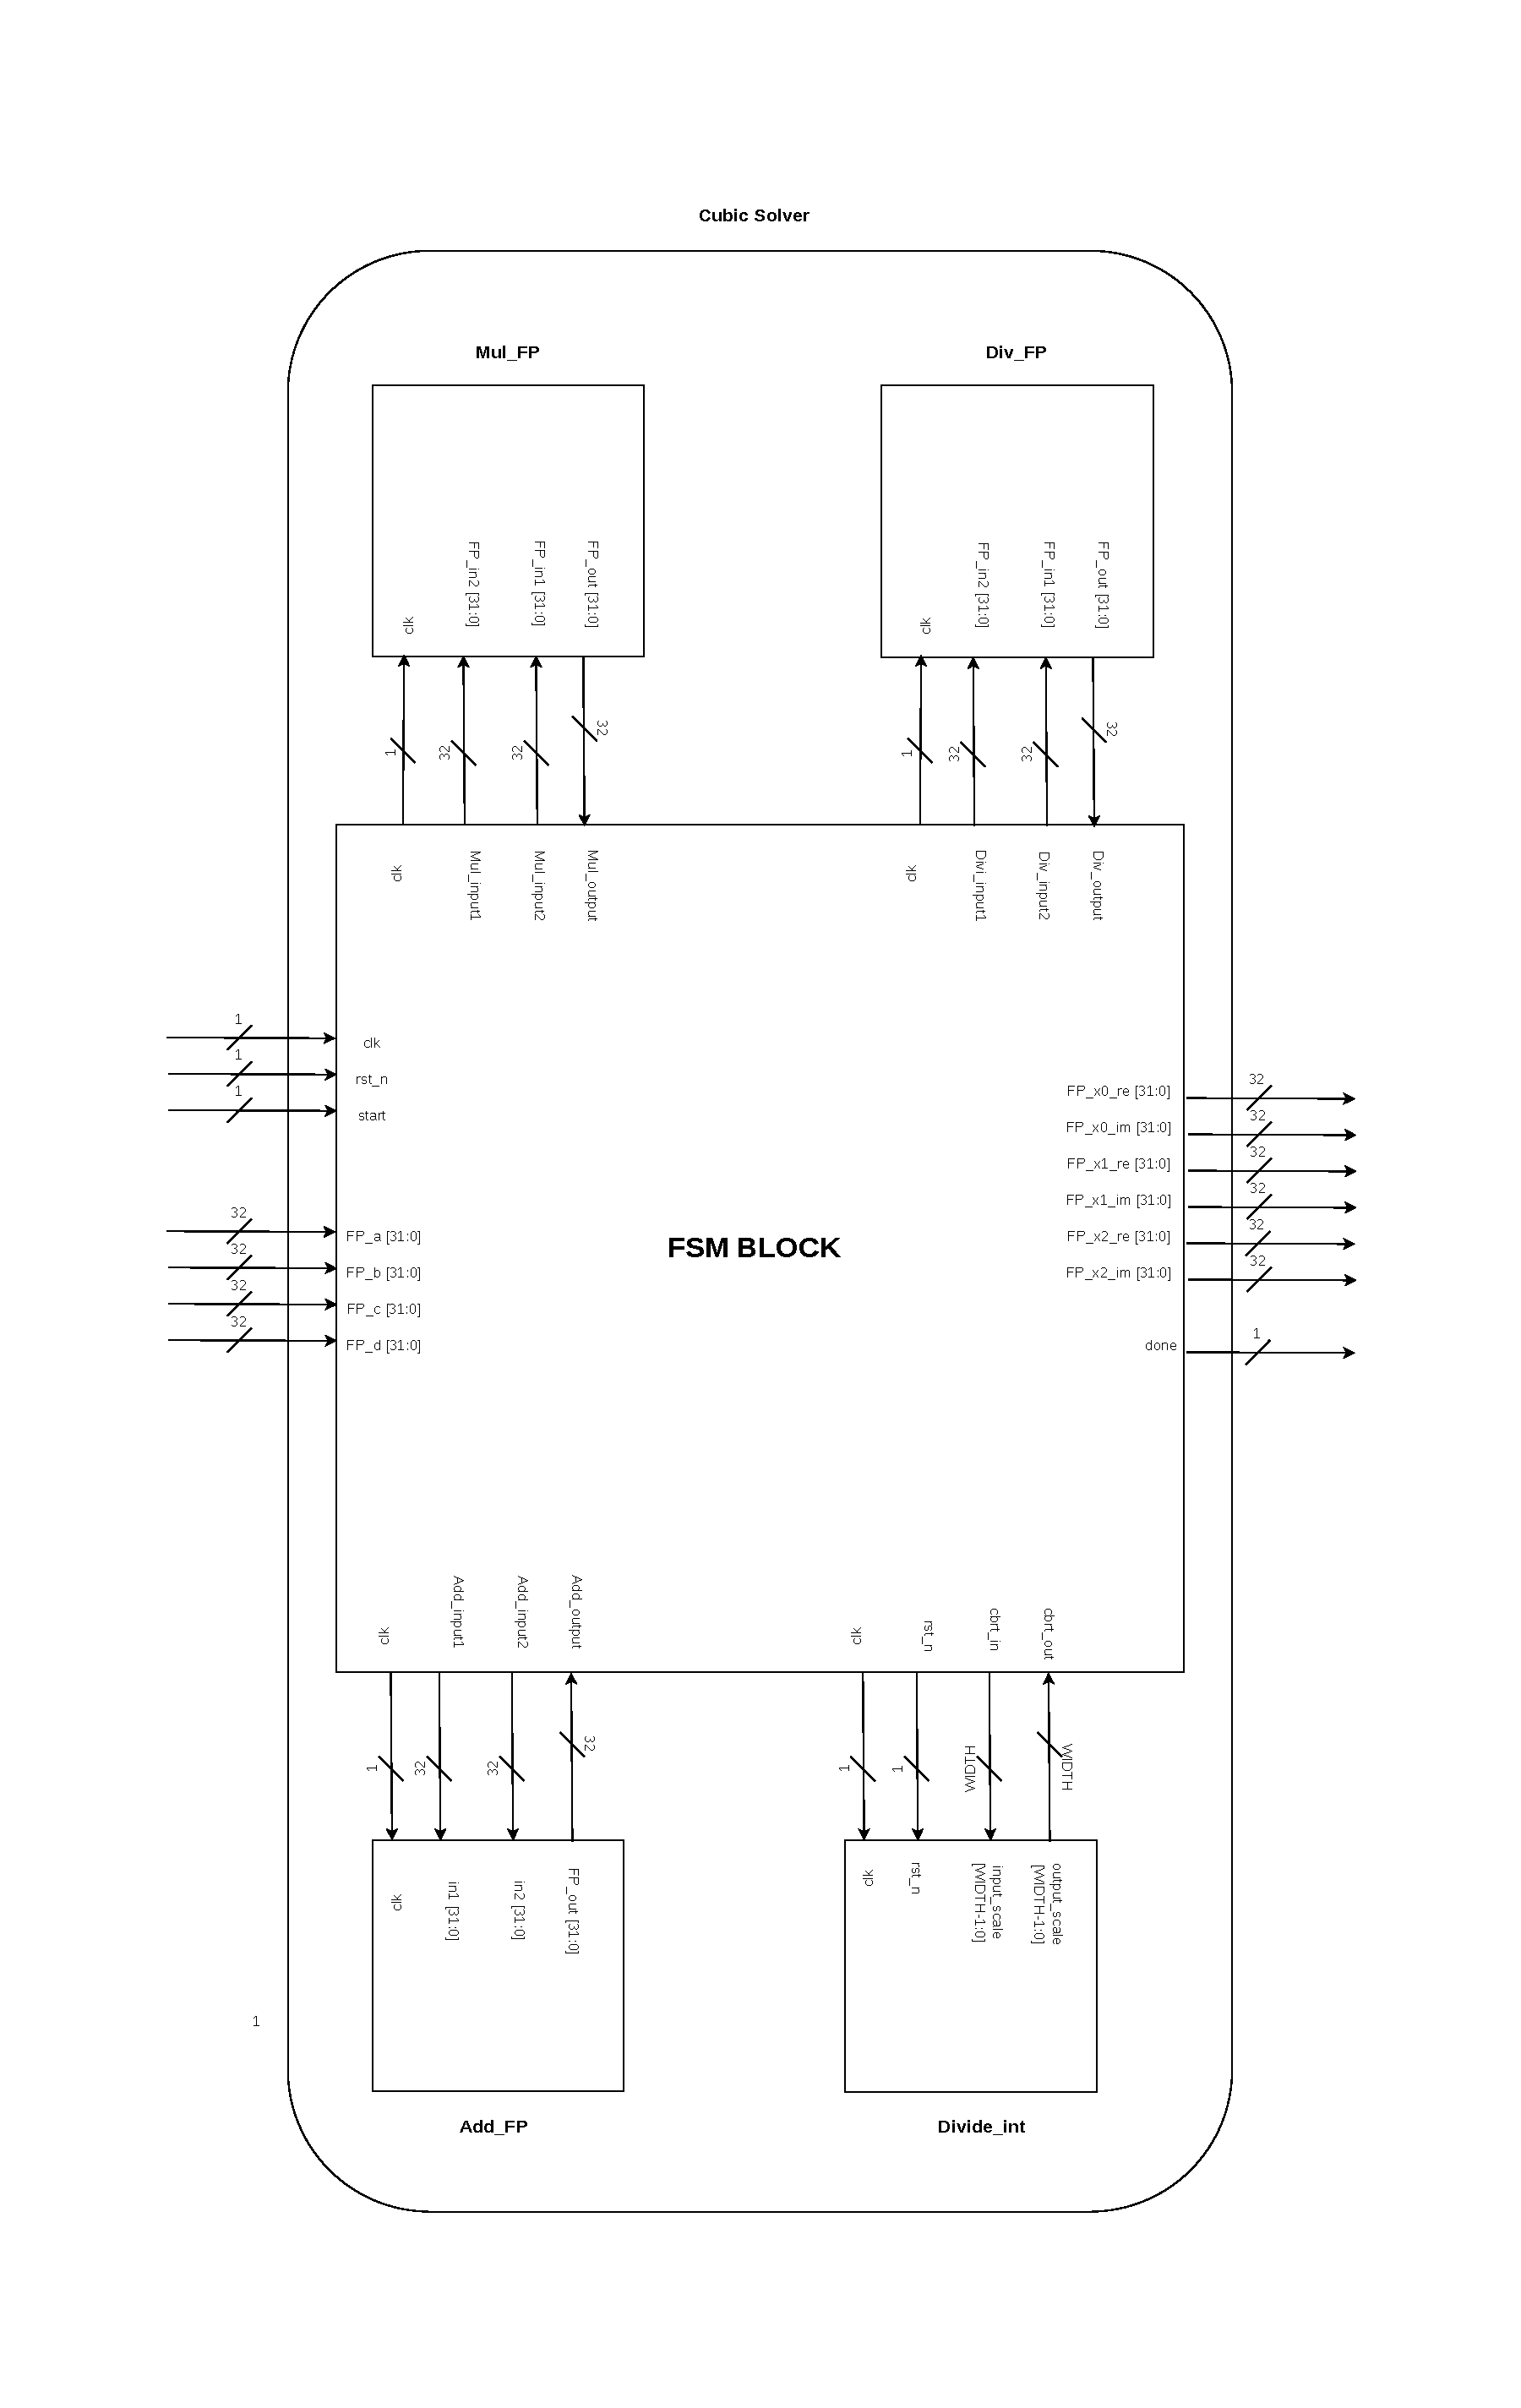
\includegraphics[width=0.70\linewidth]{graphics/Cubic_Solver.pdf}
    \caption{Internal structure of the \texttt{Cubic\_Solver} module.}
    \label{fig:cubic_solver_internal}
\end{figure}

The hardware is organized around one shared arithmetic datapath and one supervisory finite state machine. The datapath contains three floating-point operators, a small exponent-scaling helper for cube-root initialization, and a register bank for intermediate values. The controller then issues operands to the arithmetic blocks according to a cycle-by-cycle schedule encoded by \texttt{delay\_count}.

\begin{table}[H]
\centering
\caption{Main internal components of the cubic-solver architecture}
\renewcommand{\arraystretch}{1.2}
\begin{tabular}{p{3.0cm} p{2.0cm} p{1.4cm} p{8.0cm}}
\toprule
\textbf{Component} & \textbf{Signal role} & \textbf{Width} & \textbf{Description} \\
\midrule
\texttt{Add\_FP} & Add/sub datapath & 32 & Shared floating-point adder used in coefficient normalization, discriminant evaluation, Pad\'e iteration, and final root composition. \\
\texttt{Mul\_FP} & Multiply datapath & 32 & Shared floating-point multiplier used for powers, scaled terms, and complex arithmetic. \\
\texttt{Div\_FP} & Divide datapath & 32 & Shared floating-point divider used in normalization and iterative updates. \\
\texttt{Divide\_int} & Exponent helper & 8 & Approximates exponent scaling for the cube-root initial estimate. \\
\texttt{r\_temp[0:63]} & Scratch register bank & 32 & Stores partial results from pipeline outputs so later delay slots can reuse them. \\
\texttt{state}/\texttt{next\_state} & FSM controller & 4 & Controls the macro-phase of the algorithm. \\
\texttt{delay\_count} & Micro-scheduler & 7 & Aligns operator inputs with the latency of shared arithmetic units. \\
\texttt{iteration\_count} & Iteration tracker & 5 & Counts the number of Pad\'e updates performed. \\
\bottomrule
\end{tabular}
\end{table}

\subsection{Internal implementation of the arithmetic modules}

\subsubsection{\texttt{Add\_FP}}

\begin{figure}[H]
    \centering
    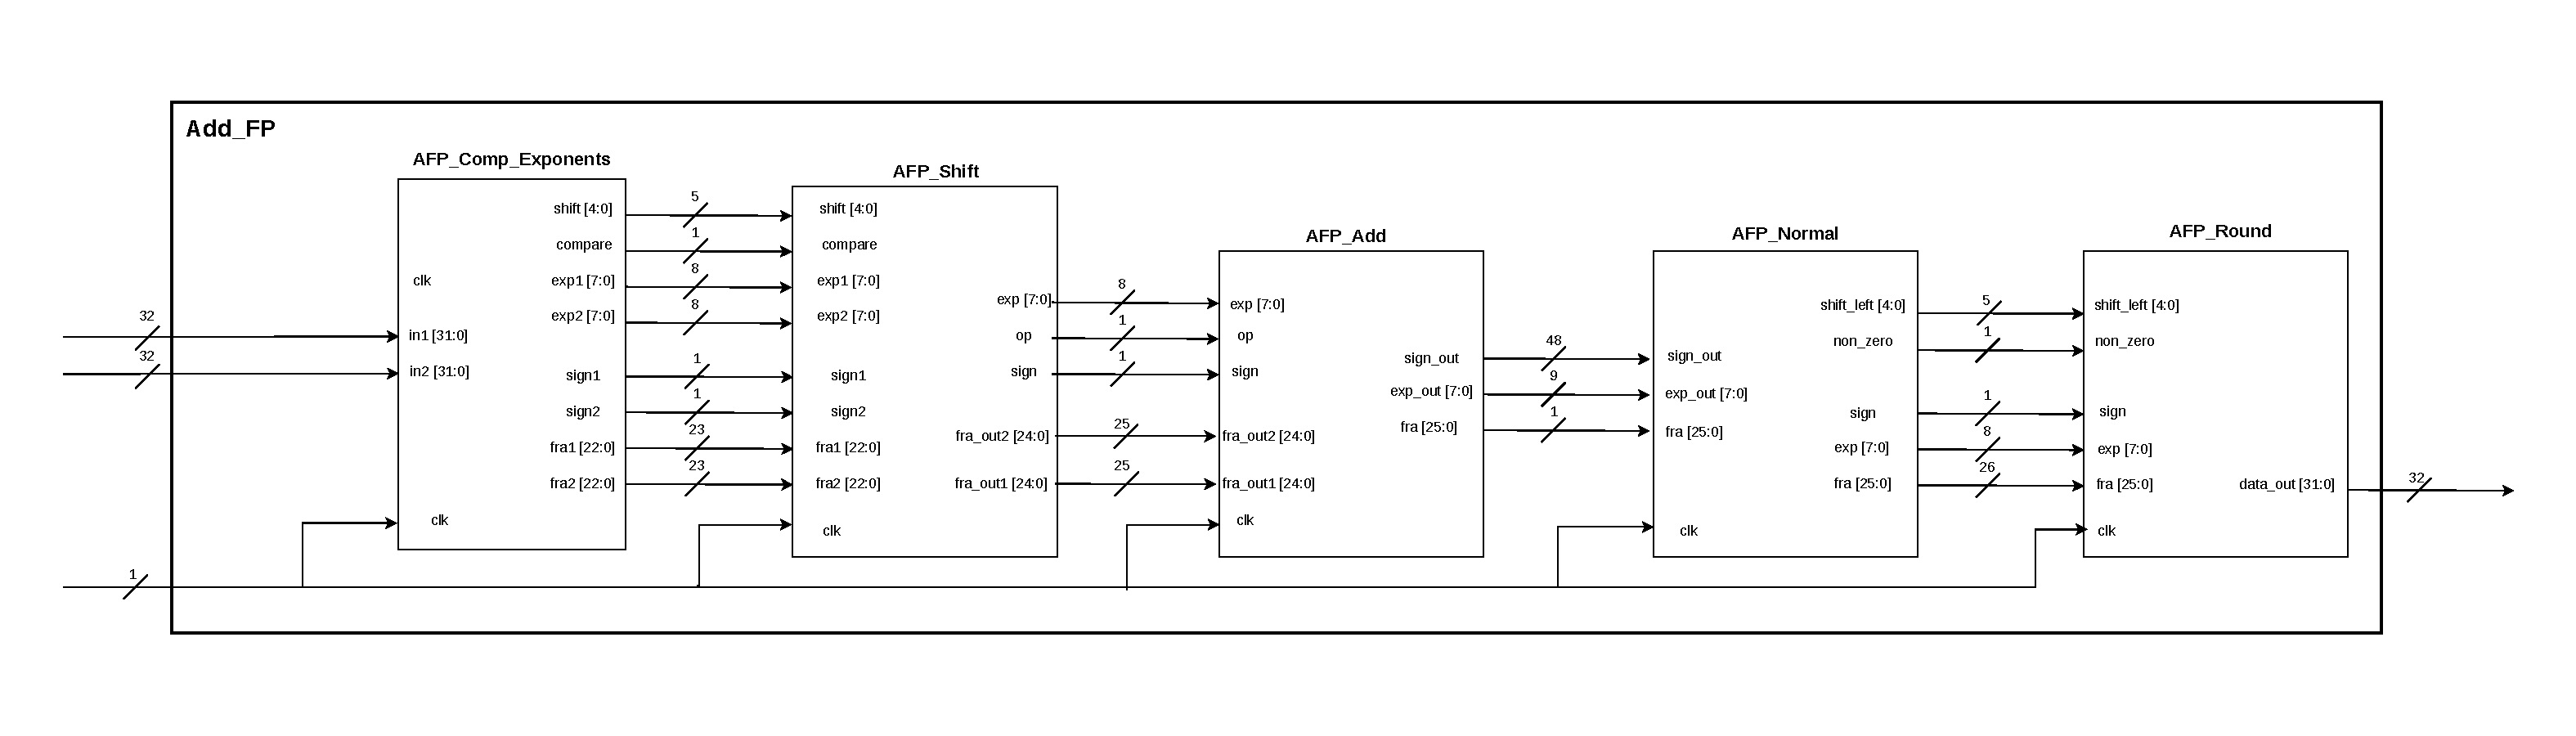
\includegraphics[width=0.95\linewidth]{graphics/Add_FP.pdf}
    \caption{Internal structure of the \texttt{Add\_FP} pipeline.}
    \label{fig:add_internal}
\end{figure}

The proposed floating-point adder is compliant with the IEEE-754 single-precision format and is implemented as a 5-stage pipeline. Instead of performing all operations in one large combinational block, the datapath is decomposed into smaller functional stages so that alignment, arithmetic, and normalization can be handled in an orderly and timing-friendly manner. The operation of each stage is summarized as follows:
\begin{itemize}
    \item \textbf{Stage 1: Exponent Comparison (\texttt{AFP\_Compare\_Exponents}).} This stage compares the exponent fields of the two operands and computes the absolute exponent difference
    \begin{equation}
        \delta = |E_A - E_B|
    \end{equation}
    to determine the alignment shift amount. At the same time, it identifies which operand has the larger exponent, preserves the sign bits, and forwards the fraction fields to the next stage.

    \item \textbf{Stage 2: Mantissa Alignment (\texttt{AFP\_Shift}).} The significand of the smaller operand is right-shifted by $\delta$ positions so that both operands share the same binary-point position. The larger operand is passed forward without loss of significance. Internally, this stage also forms the effective operation mode
    \begin{equation}
        \texttt{op} = S_A \oplus S_B
    \end{equation}
    so that the next stage knows whether the mantissas must be added or subtracted.

    \item \textbf{Stage 3: Arithmetic Operation (\texttt{AFP\_Add}).} The aligned mantissas are combined according to the effective operation sign. Functionally, this stage evaluates
    \begin{equation}
        M_{sum} = M_{large} \pm M_{shifted}
    \end{equation}
    and then converts the result back into sign-magnitude form. If the subtraction result is negative, the sign is inverted and the magnitude is stored as a positive number to simplify normalization.

    \item \textbf{Stage 4: Normalization Detection (\texttt{AFP\_Normal}).} This stage determines whether the arithmetic result is already normalized. In subtraction cases, leading zeros may appear at the MSB side of the mantissa. A priority encoder is therefore used to detect the position of the leading one and to compute the left-shift amount needed to restore the format
    \begin{equation}
        1.xxxxx
    \end{equation}
    expected by IEEE-754.

    \item \textbf{Stage 5: Normalization and Packing (\texttt{AFP\_Rounding}).} The mantissa is shifted according to the result of Stage 4, and the exponent is adjusted accordingly. If an overflow carry exists, the exponent is incremented; otherwise, it is reduced by the normalization shift amount. Finally, the result is packed back into a 32-bit IEEE-754 word.
\end{itemize}

This 5-stage organization is particularly suitable for the cubic solver because the top-level controller repeatedly issues additions such as $\Delta_0 = b^2 + c$, $\Delta = \Delta_1^2 - 4\Delta_0^3$, or the accumulation terms required by the Pad\'e iterations. A deeply regular pipeline therefore gives both structural clarity and predictable timing.

\subsubsection{\texttt{Mul\_FP}}

\begin{figure}[H]
    \centering
    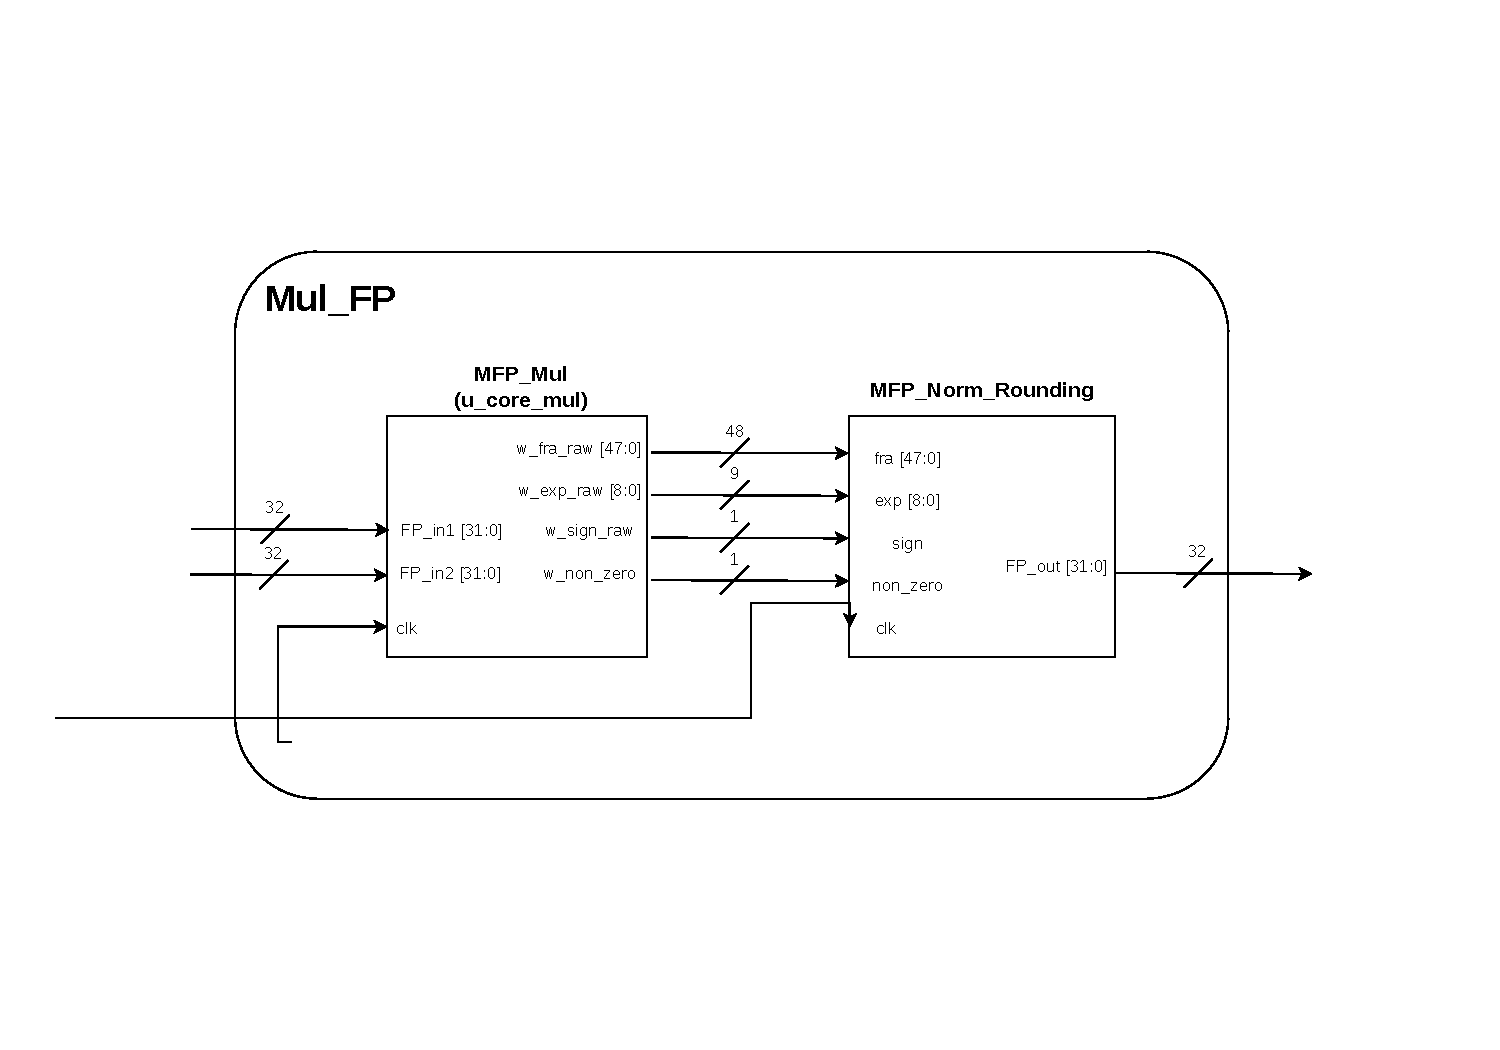
\includegraphics[width=0.92\linewidth]{graphics/Mul_FP.pdf}
    \caption{Top-level structure of the \texttt{Mul\_FP} module.}
    \label{fig:mul_internal}
\end{figure}

\begin{figure}[H]
    \centering
    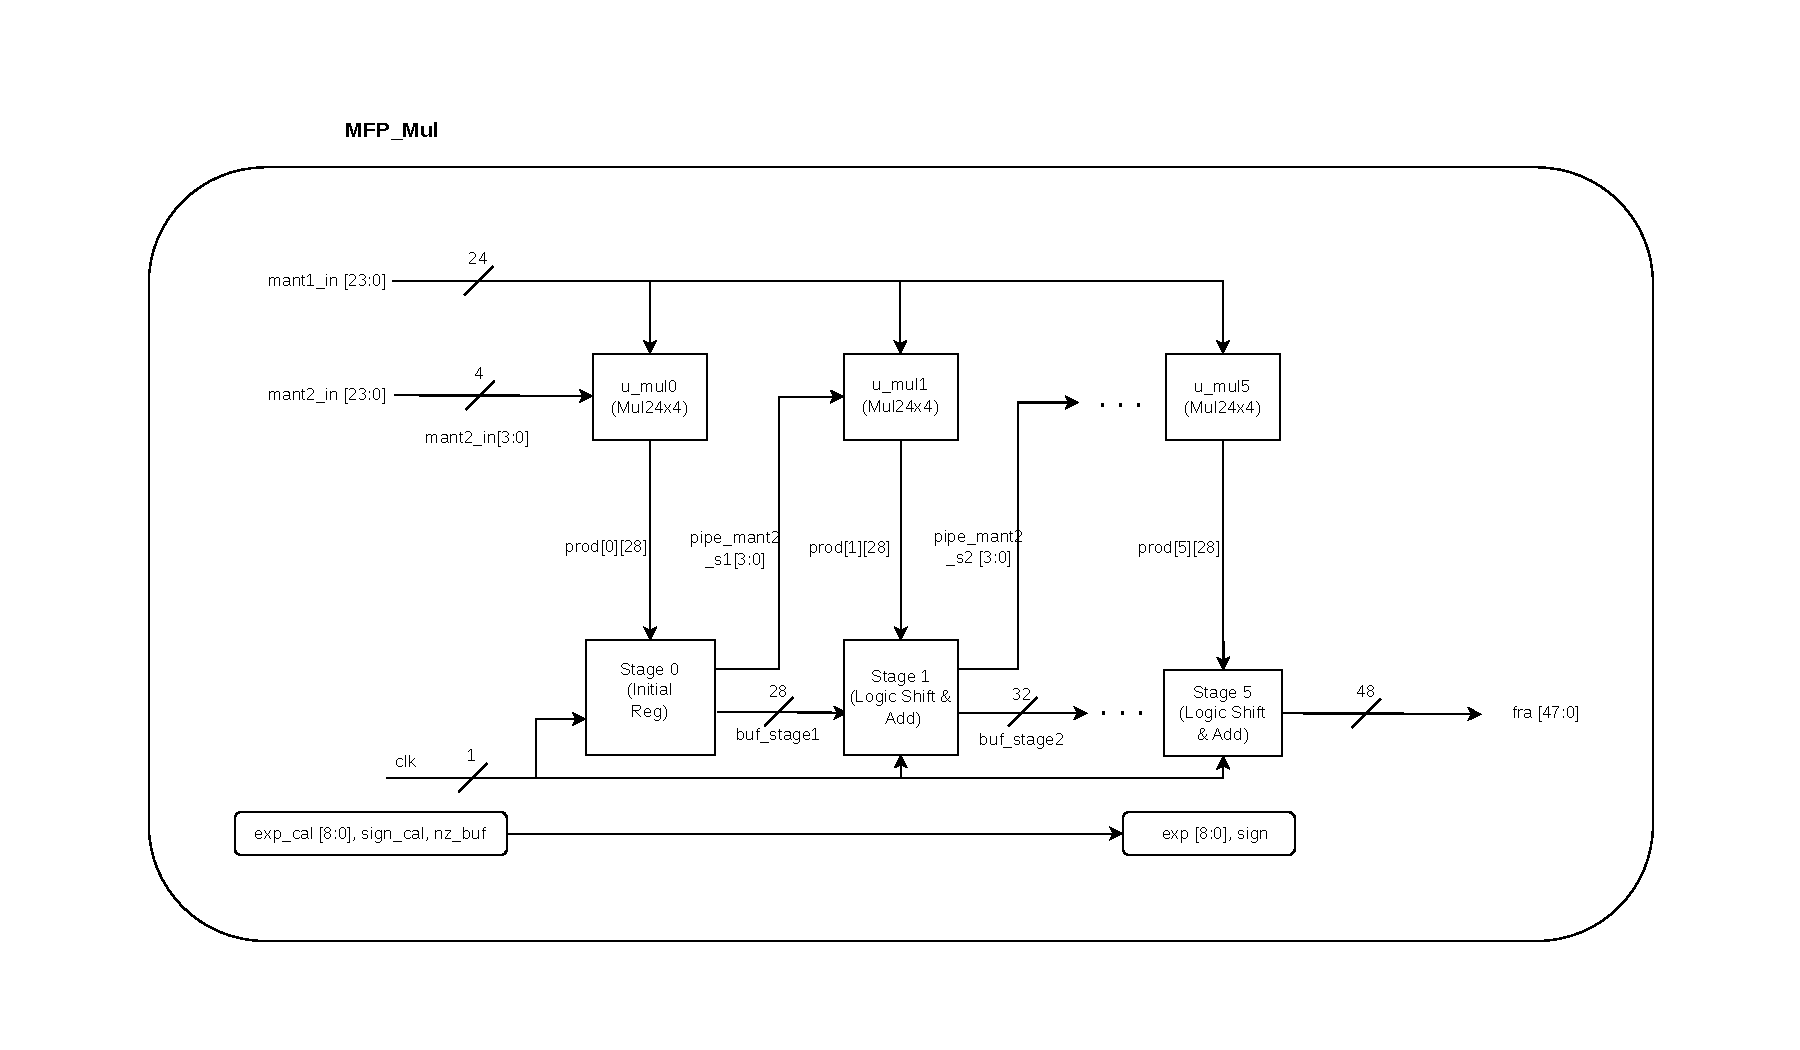
\includegraphics[width=0.92\linewidth]{graphics/MFP_Mul.pdf}
    \caption{Mantissa-multiplication core used by \texttt{Mul\_FP}.}
    \label{fig:mfp_mul_internal}
\end{figure}

To maintain high throughput and keep the critical path short, the multiplier avoids a single-cycle 24$\times$24-bit mantissa multiplication. Instead, the architecture uses a staged 4-bit nibble-decomposition strategy. The complete \texttt{Mul\_FP} block can therefore be understood as a 7-stage pipeline: 6 stages for mantissa partial-product accumulation and 1 stage for normalization and final packing.

\paragraph{Pre-processing}
Before mantissa multiplication begins, the two FP32 operands are decomposed into sign, exponent, and fraction fields. The hidden bit is appended to both fractions to form
\begin{equation}
M_A = \{1, frac_A\}, \qquad M_B = \{1, frac_B\}
\end{equation}
The tentative exponent is computed as
\begin{equation}
E_{raw} = E_A + E_B - 127
\end{equation}
and the output sign is obtained by XOR:
\begin{equation}
S_{out} = S_A \oplus S_B
\end{equation}

\paragraph{Partial Product Accumulation (Stages 1--6)}
The core multiplication logic decomposes the 24-bit multiplier mantissa into six 4-bit nibbles. In each stage $i$ ($i = 0 \dots 5$), one \texttt{Mul24x4} block computes a 24$\times$4-bit partial product, and this new contribution is accumulated with the previously stored partial sum. Conceptually, the recurrence can be interpreted as
\begin{equation}
P_i = (P_{i-1} \ll 4) + \left(M_A \times M_B[4i+3:4i]\right)
\end{equation}
where each nibble contributes one radix-$2^4$ digit of the final mantissa product.

The stage-by-stage meaning is:
\begin{itemize}
    \item \textbf{Stage 1:} use \texttt{mant2\_in[3:0]} and store the first partial product in \texttt{buf\_stage1}.
    \item \textbf{Stage 2:} use the next nibble and accumulate into \texttt{buf\_stage2}.
    \item \textbf{Stage 3:} accumulate the contribution of bits \texttt{[11:8]} into \texttt{buf\_stage3}.
    \item \textbf{Stage 4:} accumulate the contribution of bits \texttt{[15:12]} into \texttt{buf\_stage4}.
    \item \textbf{Stage 5:} accumulate the contribution of bits \texttt{[19:16]} into \texttt{buf\_stage5}.
    \item \textbf{Stage 6:} accumulate the final nibble \texttt{[23:20]} and generate the full 48-bit raw product \texttt{fra}.
\end{itemize}

This nibble-based organization ensures that the combinational depth of each stage remains shallow. Instead of building a large and timing-expensive multiplier tree, the architecture spreads the work across several short pipeline stages.

\paragraph{Normalization and Final Packaging (Final Stage)}
Once the raw 48-bit product has been formed, the block \texttt{MFP\_Norm\_Rounding} performs IEEE-754 post-processing:
\begin{itemize}
    \item \textbf{Normalization:} The block checks whether the most significant bit of the 48-bit raw product is already in normalized position. Depending on that condition, it selects either \texttt{fra[46:23]} or \texttt{fra[45:22]} as the normalized mantissa slice and updates the exponent.
    \item \textbf{Rounding:} The least significant dropped bit is used to realize round-to-nearest behavior before the final 23-bit fraction is stored.
    \item \textbf{Packing:} The sign, normalized exponent, and rounded mantissa are concatenated into the final FP32 result.
\end{itemize}

This architecture is efficient for the current application because the solver repeatedly needs products such as $\hat{b}^2$, $\hat{b}^3$, $\Delta_0^3$, $\Delta_1^2$, and the large set of cross-products required by the complex cube-root branch.

\subsubsection{\texttt{Div\_FP}}

\begin{figure}[H]
    \centering
    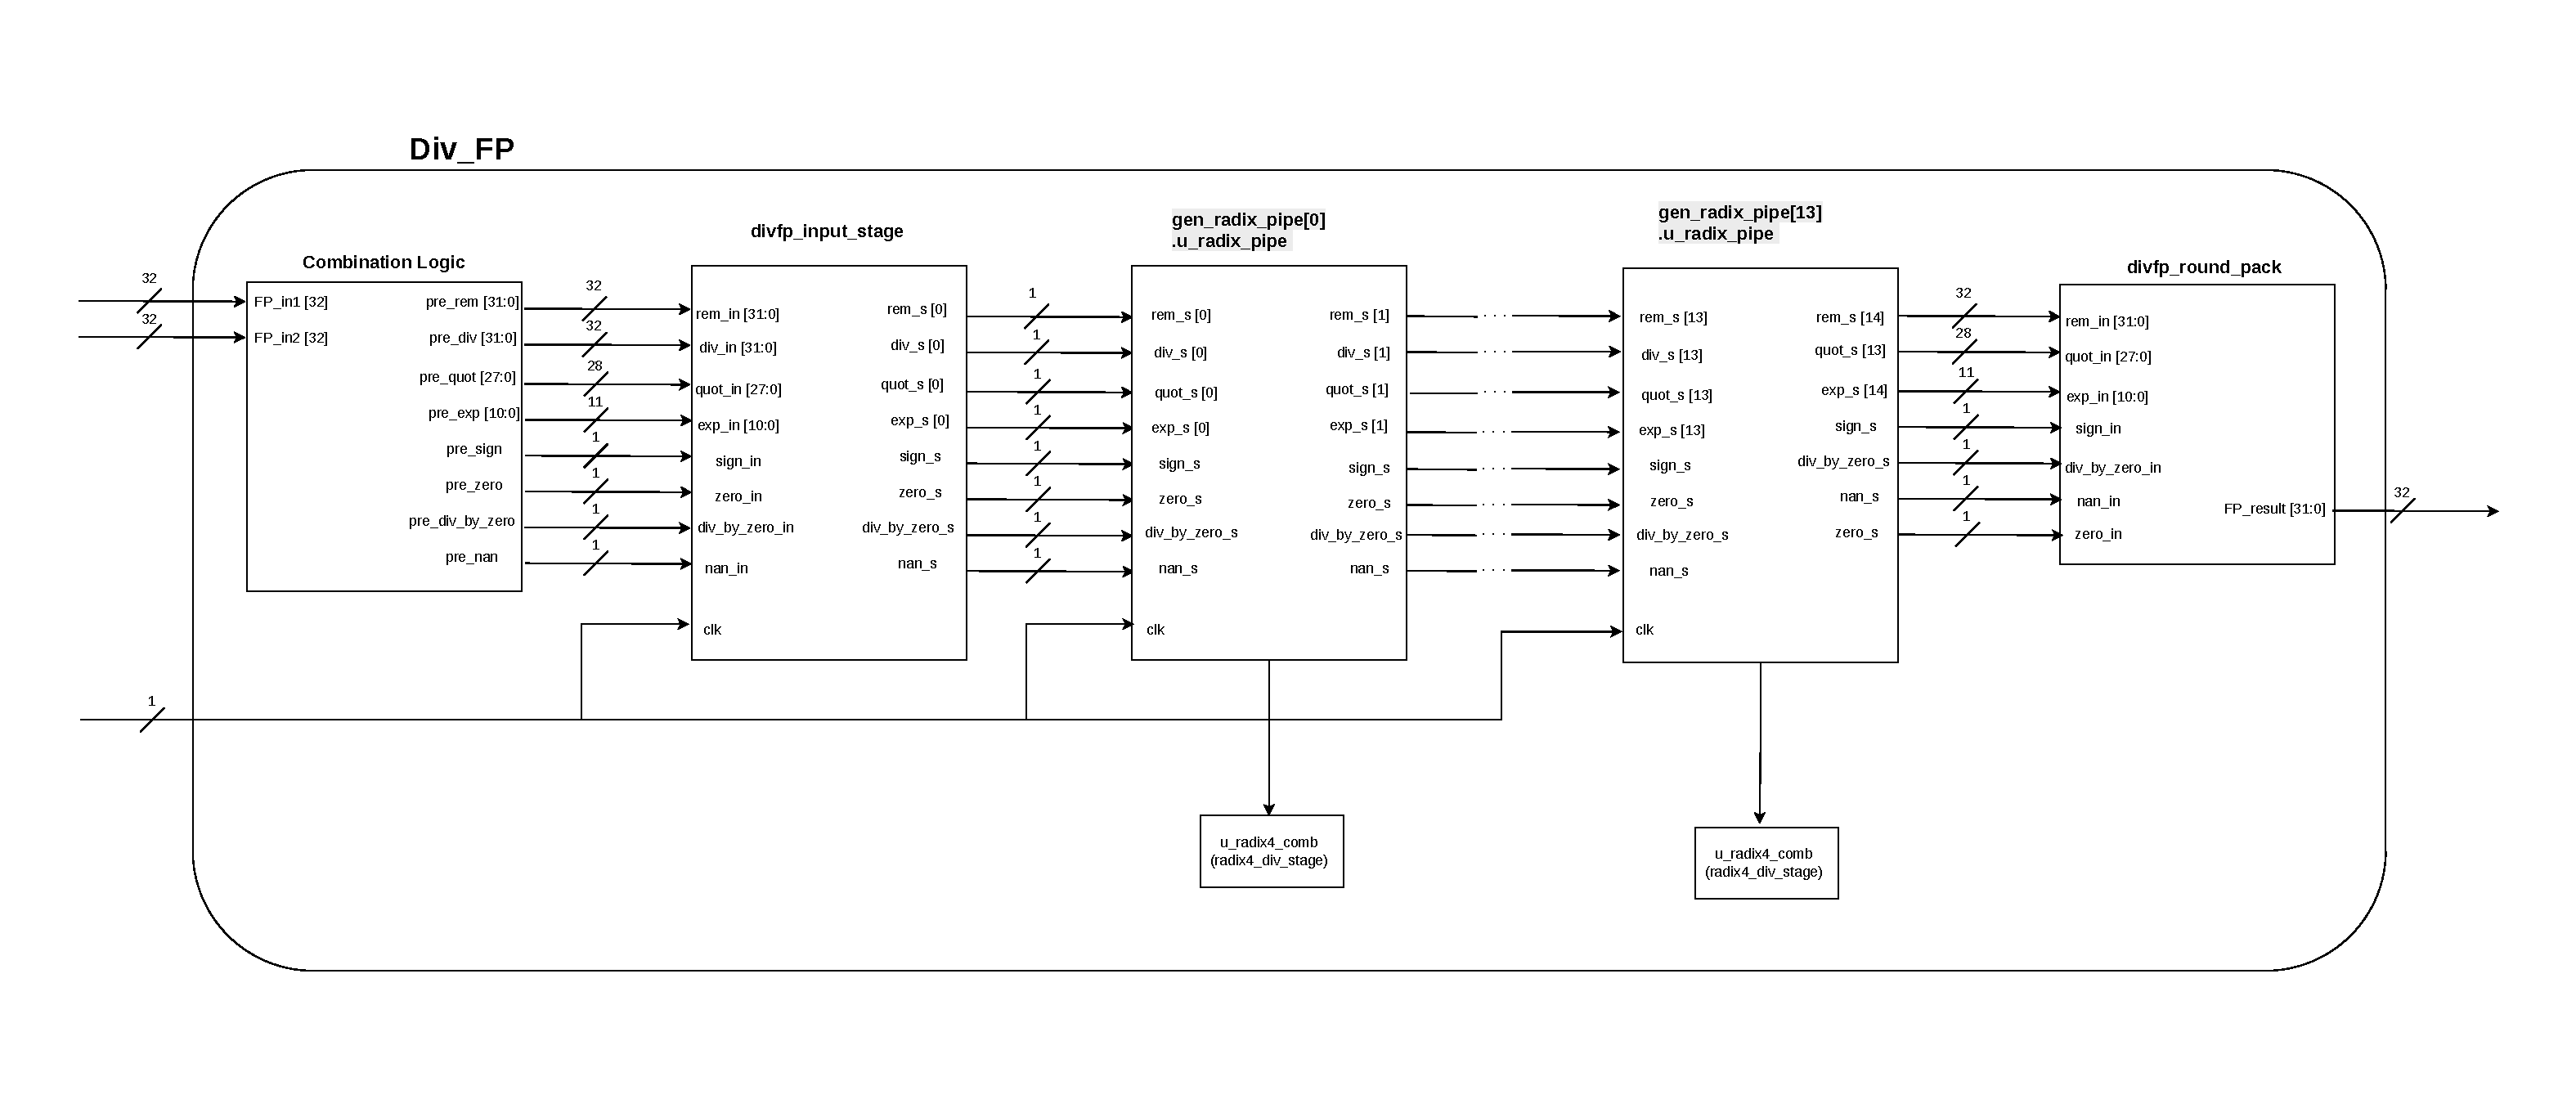
\includegraphics[width=0.95\linewidth]{graphics/Div_FP.pdf}
    \caption{Internal structure of the \texttt{Div\_FP} module.}
    \label{fig:div_internal}
\end{figure}

The division unit is designed as a radix-4 pipelined floating-point divider. Similar to the multiplier, the goal is not minimum latency in a single cycle, but rather a regular multi-stage implementation with deterministic throughput and timing behavior. The full \texttt{Div\_FP} datapath can be interpreted as a 16-cycle pipeline: 1 input stage, 14 radix-4 quotient-generation stages, and 1 output register stage.

\paragraph{Stage 1: Pre-processing and operand standardization}
The first step extracts sign, exponent, and fraction fields from the two FP32 operands. The divider then classifies special cases:
\begin{itemize}
    \item zero numerator
    \item zero denominator
    \item NaN / special exponent cases
\end{itemize}
The output sign is computed as
\begin{equation}
S_{out} = S_A \oplus S_B
\end{equation}
and the initial exponent is formed from the exponent difference between dividend and divisor. To ensure that the mantissa quotient starts in normalized range, the design compares the two mantissas:
\begin{itemize}
    \item if $M_A < M_B$, the dividend mantissa is left-shifted and the exponent is biased by 126
    \item otherwise, the mantissa is used directly and the exponent is biased by 127
\end{itemize}
This step creates the initial remainder \texttt{pre\_rem}, divisor \texttt{pre\_div}, quotient register \texttt{pre\_quot}, and exponent \texttt{pre\_exp}.

\paragraph{Stage 2: Input pipeline register}
The standardized division operands are stored in \texttt{divfp\_input\_stage}. This stage isolates the combinational preprocessing logic from the iterative radix-4 quotient datapath and guarantees synchronous propagation of the control metadata such as sign, zero flag, division-by-zero flag, and NaN flag.

\paragraph{Stages 3--16: Radix-4 quotient generation}
The main body of the divider consists of fourteen identical registered radix-4 stages. In each stage, the combinational block \texttt{radix4\_div\_stage} performs the following operations:
\begin{itemize}
    \item shift the current remainder left by 2 bits
    \item compare the shifted remainder with $2D$ and $D$
    \item subtract the largest possible multiple without making the remainder negative
    \item emit one quotient digit \texttt{q\_digit} in radix-4, equivalent to two binary quotient bits
\end{itemize}

If the stage remainder is denoted by $R_i$ and the divisor by $D$, then each stage evaluates
\begin{equation}
R_i' = 4R_i
\end{equation}
and chooses a quotient digit $q_i \in \{0,1,2,3\}$ such that
\begin{equation}
R_{i+1} = 4R_i - q_iD
\end{equation}
remains non-negative. The digit is appended into the running quotient register. Since each stage contributes two quotient bits, fourteen stages are sufficient to build a 28-bit quotient representation.

\paragraph{Final stage: Rounding and IEEE-754 packaging}
After the last radix-4 stage, the block \texttt{divfp\_round\_pack} reconstructs the floating-point result:
\begin{itemize}
    \item the quotient bits are converted into a normalized mantissa candidate
    \item guard, round, and sticky information are used to implement round-to-nearest
    \item the exponent is corrected if the rounding operation produces mantissa overflow
    \item special conditions such as NaN, division by zero, overflow, and underflow are handled before final packing
\end{itemize}
The result is then registered once more into \texttt{FP\_out}, completing the division pipeline.

The fixed latency of this divider is particularly important for the cubic solver. Since the top-level design contains only one instance of \texttt{Div\_FP}, the FSM must know exactly when a valid quotient becomes available. The regular 16-cycle structure is therefore a major advantage for state scheduling.

\subsection{Finite state machine}

\begin{figure}[H]
    \centering
    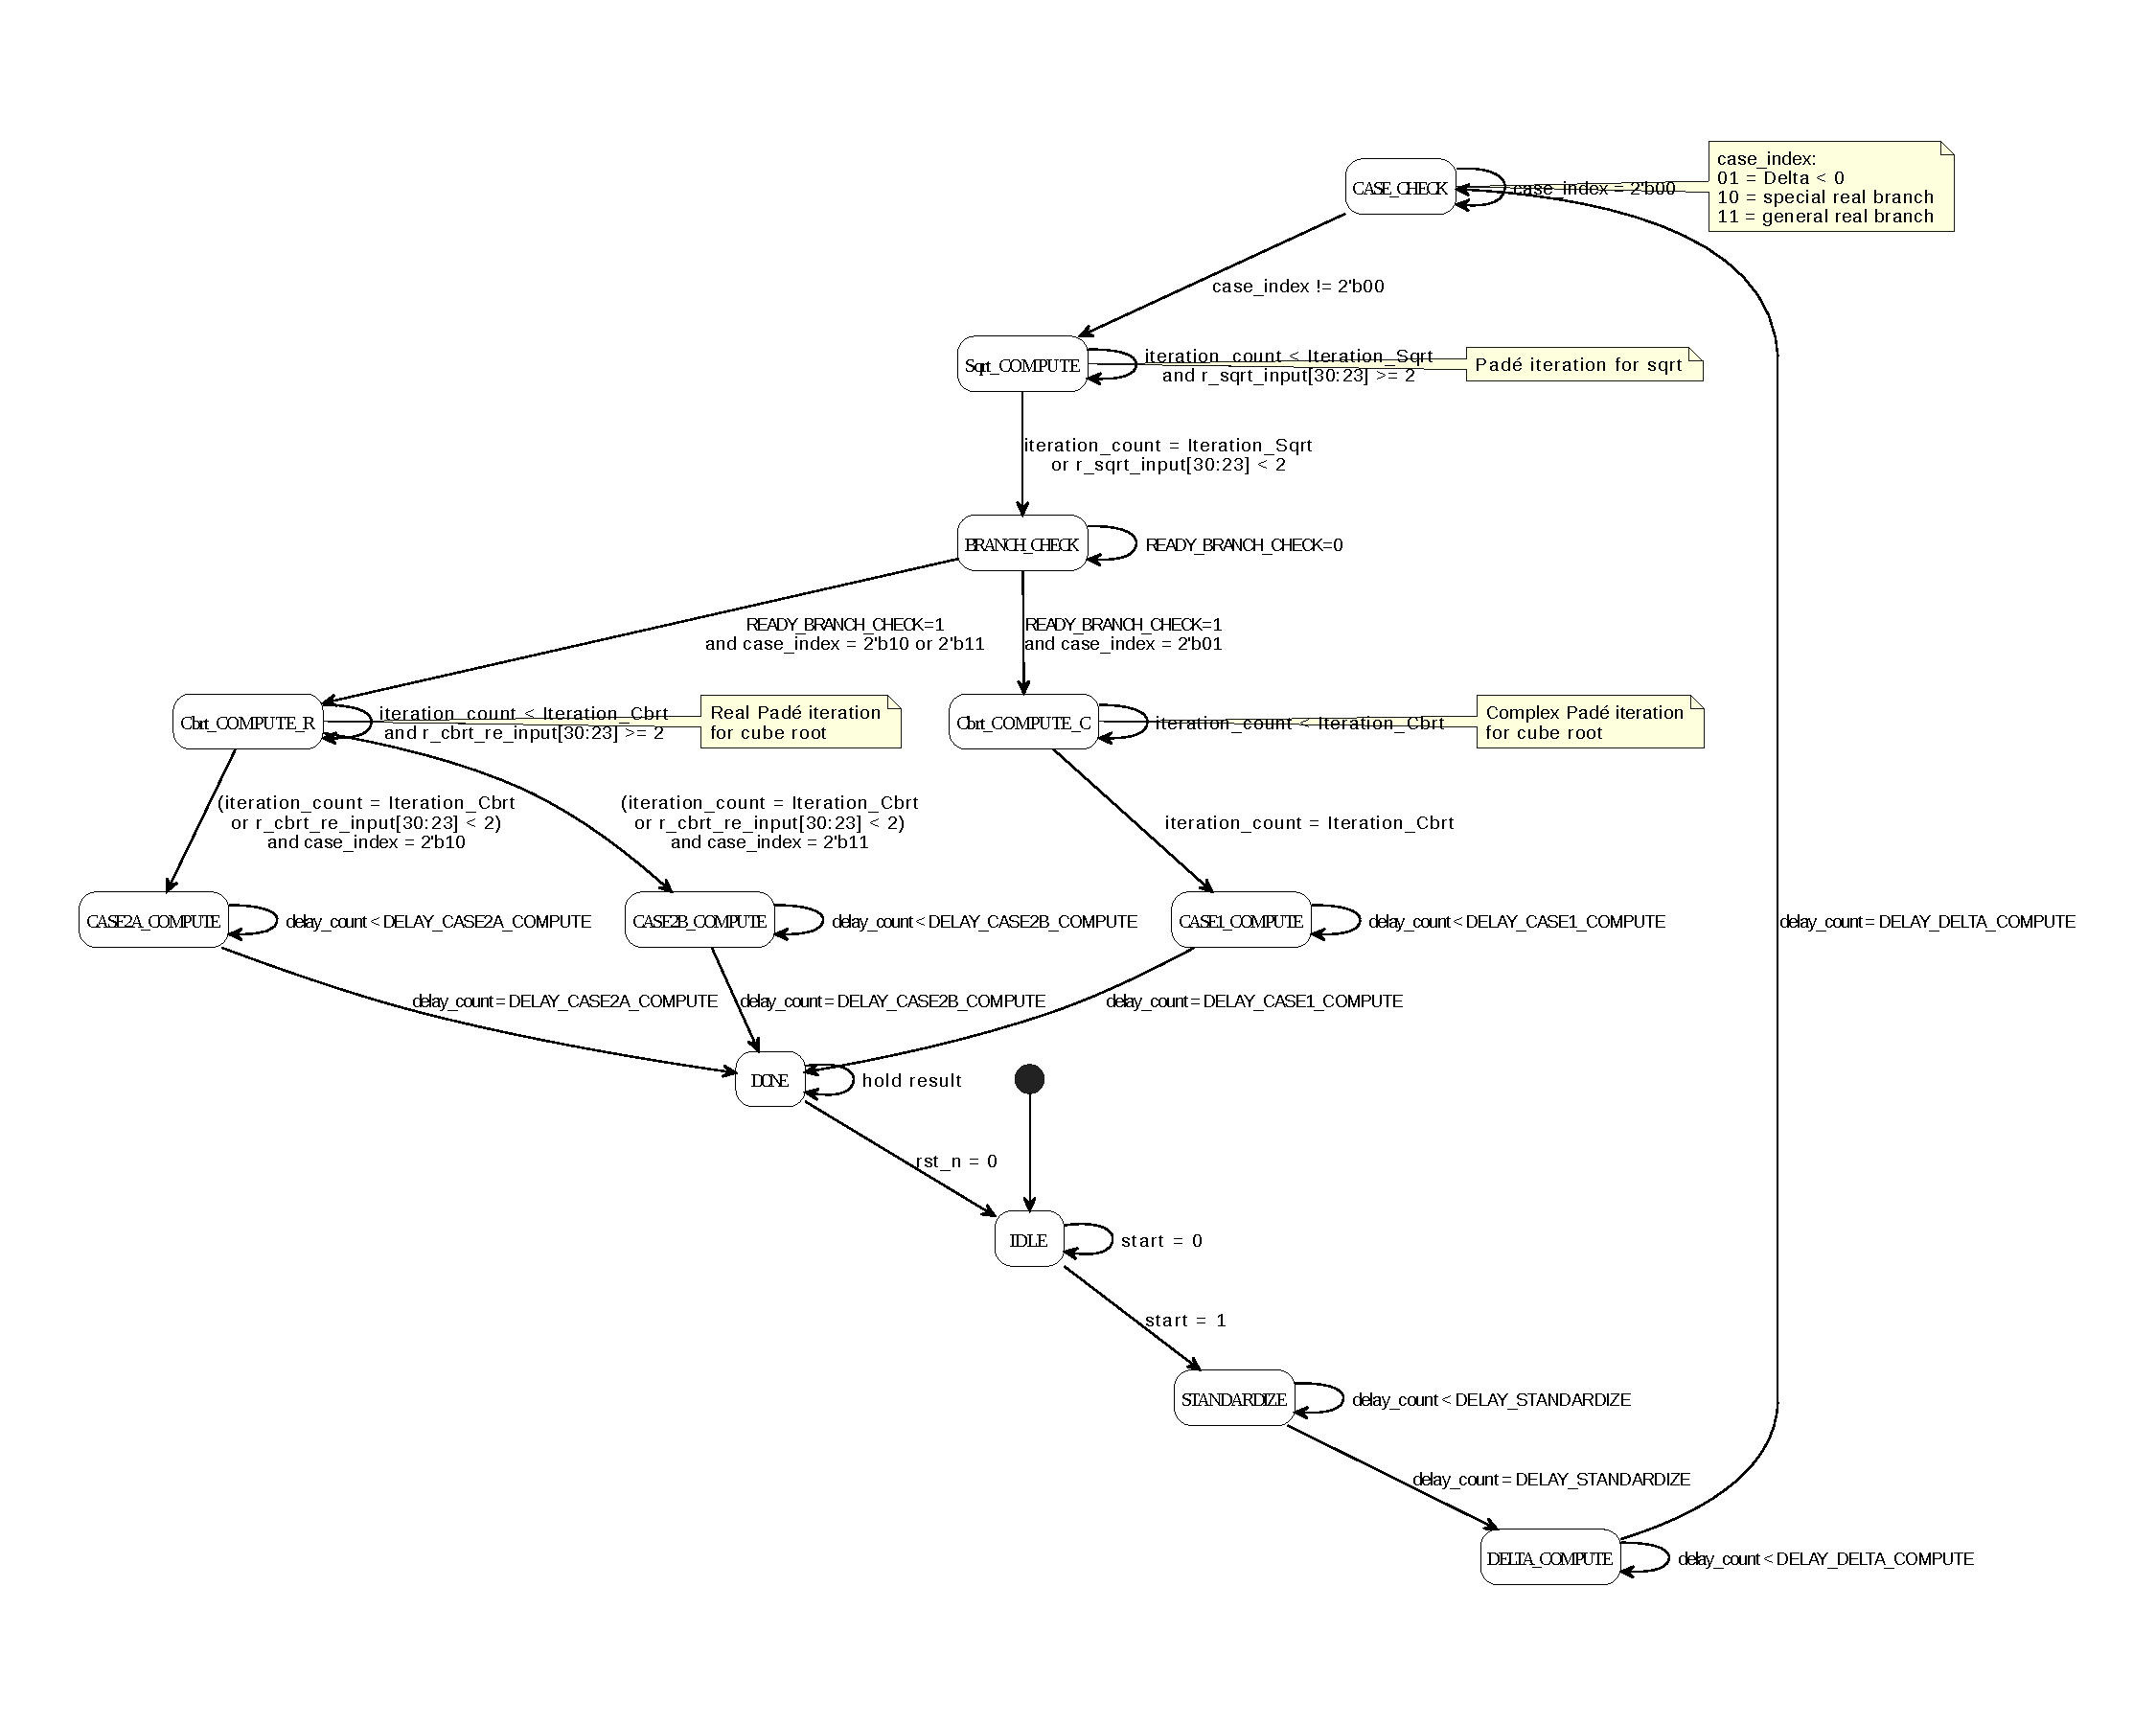
\includegraphics[width=0.95\linewidth]{graphics/FSM.pdf}
    \caption{Finite state machine of the \texttt{Cubic\_Solver} module.}
    \label{fig:cubic_solver_fsm}
\end{figure}

\subsubsection{State summary}

\begin{table}[H]
\centering
\caption{State encoding and role of the main solver FSM}
\renewcommand{\arraystretch}{1.2}
\begin{tabular}{lll p{7.8cm}}
\toprule
\textbf{State} & \textbf{Code} & \textbf{Phase} & \textbf{Main responsibility} \\
\midrule
\texttt{IDLE} & \texttt{4'b0000} & Wait & Wait for \texttt{start}, capture input coefficients, and initialize counters. \\
\texttt{STANDARDIZE} & \texttt{4'b0001} & Pre-process & Compute normalized coefficients by dividing $b$, $c$, and $d$ by $-3a$. \\
\texttt{DELTA\_COMPUTE} & \texttt{4'b0010} & Invariant generation & Compute $\Delta_0$, $\Delta_1$, and $\Delta$. \\
\texttt{CASE\_CHECK} & \texttt{4'b0011} & Branch selection & Encode the solving branch into \texttt{case\_index} and initialize the square-root stage. \\
\texttt{Sqrt\_COMPUTE} & \texttt{4'b0100} & Iteration & Run Pad\'e square-root iteration. \\
\texttt{BRANCH\_CHECK} & \texttt{4'b0101} & Dispatch & Prepare cube-root inputs and initial estimates for the chosen branch. \\
\texttt{Cbrt\_COMPUTE\_R} & \texttt{4'b0110} & Iteration & Run the real cube-root Pad\'e iteration. \\
\texttt{Cbrt\_COMPUTE\_C} & \texttt{4'b0111} & Iteration & Run the complex cube-root Pad\'e iteration. \\
\texttt{CASE1\_COMPUTE} & \texttt{4'b1000} & Output synthesis & Generate roots for the negative-discriminant branch. \\
\texttt{CASE2A\_COMPUTE} & \texttt{4'b1001} & Output synthesis & Generate roots for the simplified real branch. \\
\texttt{CASE2B\_COMPUTE} & \texttt{4'b1010} & Output synthesis & Generate roots for the general real branch. \\
\texttt{DONE} & \texttt{4'b1011} & Handshake & Assert \texttt{done} and hold valid outputs. \\
\bottomrule
\end{tabular}
\end{table}

\subsubsection{Detailed analysis of each state}

\paragraph{1. \texttt{IDLE}}
This is the reset and wait state. The solver stores the external coefficients into \texttt{r\_a}, \texttt{r\_b}, \texttt{r\_c}, and \texttt{r\_d}, clears \texttt{delay\_count}, \texttt{iteration\_count}, and \texttt{case\_index}, and waits until \texttt{start = 1}. No arithmetic operator is actively driven in this state.

\paragraph{2. \texttt{STANDARDIZE}}
The controller converts the equation to the normalized form used by the mathematical model. At the beginning of the state, the solver computes $3a$ by adding \texttt{r\_a} and \texttt{2a}, where \texttt{2a} is produced by exponent shifting. The resulting term is negated and used as the divisor for three sequential divisions:
\begin{itemize}
    \item \texttt{r\_b / (-3a)}
    \item \texttt{r\_c / (-3a)}
    \item \texttt{r\_d / (-3a)}
\end{itemize}
The outputs are written back into the working coefficient registers. This state therefore converts the external polynomial description into the internal algebraic form used by all following states.

\paragraph{3. \texttt{DELTA\_COMPUTE}}
This state computes the invariants $\Delta_0$, $\Delta_1$, and $\Delta$ by a carefully scheduled sequence of multiply-add operations:
\begin{itemize}
    \item \textbf{Early slots}: compute $\hat{b}^2$ and $\hat{b}\hat{c}$.
    \item \textbf{Middle slots}: form $\Delta_0 = \hat{b}^2 + \hat{c}$ and $2\hat{b}^3 + 3\hat{b}\hat{c} + 3\hat{d}$.
    \item \textbf{Late slots}: form $\Delta_1^2$, $4\Delta_0^3$, and finally $\Delta = \Delta_1^2 - 4\Delta_0^3$.
\end{itemize}
The state stores partial results in \texttt{r\_temp[0]} and the final invariant values in \texttt{r\_delta\_0}, \texttt{r\_delta\_1}, \texttt{r\_delta\_0\_Compare}, and \texttt{r\_delta}.

\paragraph{4. \texttt{CASE\_CHECK}}
Once the discriminant terms are available, the solver decides which branch of the cubic formula must be executed next. This state is therefore the main decision point of the entire algorithm. Conceptually, the FSM divides the problem into three cases:
\begin{itemize}
    \item \textbf{Case 1 -- complex branch} (\texttt{case\_index = 2'b01}): selected when $\Delta < 0$. In this case, the hardware must interpret $\sqrt{\Delta}$ as a purely imaginary quantity and later perform a complex-valued cube-root iteration.
    \item \textbf{Case 2A -- simplified real branch} (\texttt{case\_index = 2'b10}): selected when the special repeated-root condition is detected. The subsequent cube-root stage only needs a real-valued operand derived from $\Delta_1$.
    \item \textbf{Case 2B -- general real branch} (\texttt{case\_index = 2'b11}): selected for all remaining cases. The solver must later compute both $C$ and $\Delta_0/C$ to reconstruct the final roots.
\end{itemize}

Besides selecting the branch, this state also prepares the square-root phase:
\begin{itemize}
    \item \texttt{r\_sqrt\_input} is loaded with either $\Delta$ or $-\Delta$, depending on whether the square root must be treated as real or imaginary.
    \item \texttt{r\_sqrt\_output} is initialized with \texttt{sqrt\_output\_init}, which is an exponent-based first estimate derived from the operand magnitude.
    \item \texttt{iteration\_count} is cleared so that the Pad\'e loop starts from its first iteration.
\end{itemize}
Functionally, \texttt{CASE\_CHECK} is the bridge between discriminant evaluation and the branch-specific numerical refinement process.

\paragraph{5. \texttt{Sqrt\_COMPUTE}}
This state implements the Pad\'e update for square root:
\begin{equation}
P_{n+1} = P_n \cdot \frac{P_n^2 + 3S}{3P_n^2 + S}
\end{equation}
Before the iterative loop starts, the initial estimate $P_0$ is not chosen arbitrarily. The RTL forms it by manipulating the exponent of the operand:
\begin{equation}
\texttt{sqrt\_output\_exp = ((exp(S) + 127) >> 1)}
\end{equation}
and then reconstructs a provisional FP32 value with the same mantissa field:
\begin{equation}
\texttt{sqrt\_output\_init = \{0, sqrt\_output\_exp, mantissa(S)\}}
\end{equation}
This is an exponent-based magnitude approximation to $\sqrt{S}$, and it provides a much better starting point than a constant seed.

The controller dispatches arithmetic operations over multiple delay slots:
\begin{itemize}
    \item compute $P_n^2$,
    \item compute $3S$,
    \item form $P_n^2 + 3S$ and $3P_n^2 + S$,
    \item divide the two terms after multiplying the numerator by $P_n$.
\end{itemize}
The new approximation is stored back into \texttt{r\_sqrt\_output}. The state loops until \texttt{iteration\_count} reaches \texttt{Iteration\_Sqrt} or the operand is sufficiently small.

\paragraph{6. \texttt{BRANCH\_CHECK}}
This state specializes the next phase according to \texttt{case\_index}:
\begin{itemize}
    \item For the complex branch, it forms the real and imaginary parts of $(\Delta_1 + \sqrt{\Delta})/2$ by halving \texttt{r\_delta\_1} and \texttt{r\_sqrt\_output} through exponent adjustment. The state then compares both exponents and selects the larger one as \texttt{exponent\_max} so that the complex cube-root seed has a safe magnitude.
    \item For the simplified real branch, it uses $\Delta_1$ directly as cube-root input and initializes the imaginary path to zero.
    \item For the general real branch, it first adds $\Delta_1$ and $\sqrt{\Delta}$, then divides by two to form the real cube-root input.
\end{itemize}
In all three branches, the cube-root estimate is initialized through exponent scaling rather than through a fixed numerical constant. The helper block \texttt{Divide\_int} approximates
\begin{equation}
E_{\sqrt[3]{S}} \approx 127 + \frac{E_S - 127}{3}
\end{equation}
so that the FSM can build the first cube-root estimate directly from the FP32 exponent field. The flag \texttt{READY\_BRANCH\_CHECK} is asserted when both the branch-specific operand and the corresponding initial estimate are ready, allowing the FSM to enter the correct cube-root state.

\paragraph{7. \texttt{Cbrt\_COMPUTE\_R}}
This state evaluates the real Pad\'e cube-root update
\begin{equation}
P_{n+1} = P_n \cdot \frac{P_n^3 + 2S}{2P_n^3 + S}
\end{equation}
The initial estimate $P_0$ used in this state is generated before entry by exponent scaling, not by iterative search. This means the real cube-root iteration starts from a value that already has approximately the correct order of magnitude.

The controller schedules:
\begin{itemize}
    \item $P_n^2$ and $P_n^3$,
    \item $2S$ and $2P_n^3$,
    \item the numerator and denominator sums,
    \item the final division that yields the next approximation.
\end{itemize}
At the end of the iteration budget, the result is written to \texttt{r\_C\_re} while \texttt{r\_C\_im} remains zero.

\paragraph{8. \texttt{Cbrt\_COMPUTE\_C}}
This is the most arithmetic-intensive state because it performs Pad\'e cube-root iteration on a complex operand. The state must evaluate both the numerator $P^4 + 2SP$ and the denominator $2P^3 + S$, then perform a complex division:
\begin{equation}
\frac{n_r + jn_i}{d_r + jd_i}
=
\frac{(n_rd_r + n_id_i) + j(n_id_r - n_rd_i)}{d_r^2 + d_i^2}
\end{equation}
To support this process, the controller uses a large subset of \texttt{r\_temp[]} to store partial real and imaginary products such as:
\begin{itemize}
    \item real and imaginary parts of $P^2$,
    \item real and imaginary parts of $SP$,
    \item real and imaginary parts of $P^3$ and $P^4$,
    \item the numerator and denominator of the final complex quotient.
\end{itemize}
The initial complex estimate is also generated by exponent logic. Instead of deriving separate analytical seeds for the real and imaginary parts, the hardware uses the larger exponent between both components as a conservative magnitude reference, then reconstructs FP32 seed values for \texttt{r\_cbrt\_re\_output} and \texttt{r\_cbrt\_im\_output}. This state demonstrates the main architectural idea of the project: even complex-valued iterations are realized by scheduling a small number of shared scalar FP32 arithmetic blocks.

\paragraph{9. \texttt{CASE1\_COMPUTE}}
This state generates three roots for the negative-discriminant branch. Since $C$ is complex, the solver combines \texttt{r\_C\_re}, \texttt{r\_C\_im}, and the constants $\varepsilon$ and $\varepsilon^2$ to produce
\begin{equation}
x_k = \hat{b} + \varepsilon^k C + \varepsilon^{2k}\overline{C}
\end{equation}
The outputs are written progressively into \texttt{FP\_x0\_*}, \texttt{FP\_x1\_*}, and \texttt{FP\_x2\_*} over several delay slots.

\paragraph{10. \texttt{CASE2A\_COMPUTE}}
This state handles the simplified real branch. Only one real value $C$ is needed, so the solver forms
\begin{equation}
x_k = \hat{b} + \varepsilon^k C
\end{equation}
The first root remains purely real, while the second and third roots are produced as a conjugate pair by multiplying $C$ with the real and imaginary parts of $\varepsilon$.

\paragraph{11. \texttt{CASE2B\_COMPUTE}}
This state handles the general real branch, which requires both $C$ and $\Delta_0/C$. The controller first launches the division \texttt{r\_delta\_0 / r\_C\_re}, then combines the quotient with the $\varepsilon$-scaled copies of $C$ to form:
\begin{equation}
x_k = \hat{b} + \varepsilon^k C + \varepsilon^{2k}\frac{\Delta_0}{C}
\end{equation}
Compared with \texttt{CASE2A\_COMPUTE}, this state is longer because it must wait for the divider output before the final root-reconstruction steps can be completed.

\paragraph{12. \texttt{DONE}}
The state asserts \texttt{done = 1} and holds all output roots stable. This allows the external environment to sample the results without ambiguity.

\subsection{The general operational principle of each state}

From an implementation point of view, the most important characteristic of this design is the tight coupling between FSM state and datapath issue pattern:
\begin{itemize}
    \item \textbf{State selection} determines the current algorithmic phase.
    \item \textbf{\texttt{delay\_count}} determines which arithmetic expression inside that phase is active at the current cycle.
    \item \textbf{\texttt{MulInput*}, \texttt{AddInput*}, and \texttt{DivInput*}} are assigned combinationally from the current state and delay slot.
    \item \textbf{Pipeline outputs} are sampled later into \texttt{r\_temp[]} or dedicated registers once the expected arithmetic latency has elapsed.
\end{itemize}

This means that the solver behaves like a microprogrammed datapath: the FSM chooses the algorithmic branch, while \texttt{delay\_count} plays the role of a local instruction pointer that sequences operand issue and result capture. The state-operation tables collected in the supplementary design notes show this clearly: in each state, different delay slots are assigned to specific \texttt{Mul\_FP}, \texttt{Add\_FP}, or \texttt{Div\_FP} transactions, and the resulting outputs are then written into \texttt{r\_temp[]} or into dedicated working registers such as \texttt{r\_delta}, \texttt{r\_sqrt\_output}, and \texttt{r\_C\_re}. That organization is the key reason why a relatively small set of arithmetic modules can implement a much more complex cubic-equation solver.

\section{Simulation}

\subsection{Simulation Strategy}

The Lab 3 verification flow is organized around four independent verification targets located in the \texttt{sim} folder: \texttt{tb\_Add\_FP.v}, \texttt{tb\_Mul\_FP.v}, \texttt{tb\_Div\_FP.v}, and \texttt{tb\_Cubic\_Solver\_file.v} (complemented by the direct testbench \texttt{tb\_Cubic\_Solver.v}). Each file is specifically written to exercise one floating-point component with a specialized testbench structure that matches the structural behavior of the Design Under Test (DUT). The sub-modules (adder, multiplier, and divider) are verified using continuous data streams or task-driven pipelines combined with latency-aware assertion checking. The top-level cubic solver is evaluated using a dual-track methodology: a direct testbench to inspect internal Finite State Machine (FSM) behavior across explicit mathematical boundary conditions, and a file-based closed-loop regression testbench capable of running thousands of automated randomized vectors while logging calculation traces.

To ensure comprehensive documentation, each testbench is evaluated from three distinct viewpoints:
\begin{enumerate}
    \item \textbf{Stimulus Construction:} The source, distribution, and mathematical characteristics of the input vectors.
    \item \textbf{Temporal Execution Protocol:} The cycle-by-cycle behavioral management including hardware reset assertions, non-blocking input application, latency-matching wait states, and stable output sampling.
    \item \textbf{Evaluation Criteria and Outputs:} The expected mathematical tolerance thresholds, observed console logs, pass/fail metrics, and wave capture intervals.
\end{enumerate}

\subsection{Testbench File Map}

Table~\ref{tab:testbench_file_map} provides a comprehensive map of the verification targets, their exact roles, and their testing configurations within the Lab 3 simulation environment.

\begin{table}[H]
\centering
\renewcommand{\arraystretch}{1.2}
\begin{tabular}{p{0.28\linewidth} p{0.32\linewidth} p{0.34\linewidth}}
\toprule
\textbf{Testbench File} & \textbf{Purpose} & \textbf{Verification Style} \\
\midrule
\texttt{tb\_Add\_FP.v} & Pipelined floating-point addition & Directed vectors, latency-based compare, 8-count integer LSB tolerance. \\
\texttt{tb\_Mul\_FP.v} & Pipelined floating-point multiplication & Burst stimulus, latency-based compare, strict 1-LSB rounding margin. \\
\texttt{tb\_Div\_FP.v} & Floating-point division & Task-based pipeline tests, IEEE-754 special corner cases. \\
\texttt{tb\_Cubic\_Solver.v} & Direct cubic equation validation & FSM state verification across 6 distinct mathematical edge cases. \\
\texttt{tb\_Cubic\_Solver\_file.v} & Mass batch regression & 3-phase automated closed-loop flow driven by external Python scripts. \\
\bottomrule
\end{tabular}
\caption{Testbench files used in the Lab 3 simulation flow}
\label{tab:testbench_file_map}
\end{table}

\subsection{Add\_FP Testbench}

The pipelined single-precision adder is verified using \texttt{tb\_Add\_FP.v}. This verification suite instantiates \texttt{Add\_FP} as the DUT and initializes three local memories: \texttt{test\_a}, \texttt{test\_b}, and \texttt{expected\_res}, each configured with 30 pre-calculated test vectors. These vectors are hardcoded as 32-bit single-precision hexadecimal strings conforming to the IEEE-754 standard. The system is driven by a 100 MHz clock source with a fixed period of 10 ns.

The temporal execution of the testbench is strictly split into two parallel driving and monitoring processes:
\begin{itemize}
    \item \textbf{Driver Process:} The inputs \texttt{in1} and \texttt{in2} are initialized to zero. Following a setup hold of two clock periods ($2 \times \text{PERIOD}$), a \texttt{for} loop sequentially drives the input pairs onto the DUT ports at every rising edge (\texttt{posedge clk}) utilizing non-blocking assignments (\texttt{<=}) to model a realistic upstream pipeline feed.
    \item \textbf{Monitor Process:} The verification block implements a latency-matching delay that holds evaluation for two initial setup periods plus the exact internal hardware pipeline latency of 5 clock cycles:
    $$\text{Total Wait} = (2 \times \text{PERIOD}) + (5 \times \text{PERIOD})$$
    After this delay, the monitor samples the output port \texttt{data\_out} on every subsequent rising edge. 
\end{itemize}

The evaluation block accounts for rounding divergences caused by hardware normalization or mantissa truncation. Instead of demanding absolute bit-level equality, the checker applies a numerical tolerance window allowing a difference of up to 8 integer counts at the Least Significant Bit (LSB). The simulation successfully passed all 30 directed test vectors (\textbf{PASS 30/30}), verifying structural timing and math accuracy under zero-sum cancellation ($a + (-a) = 0$) and identity operations ($a + 0 = a$).

\begin{figure}[H]
\centering
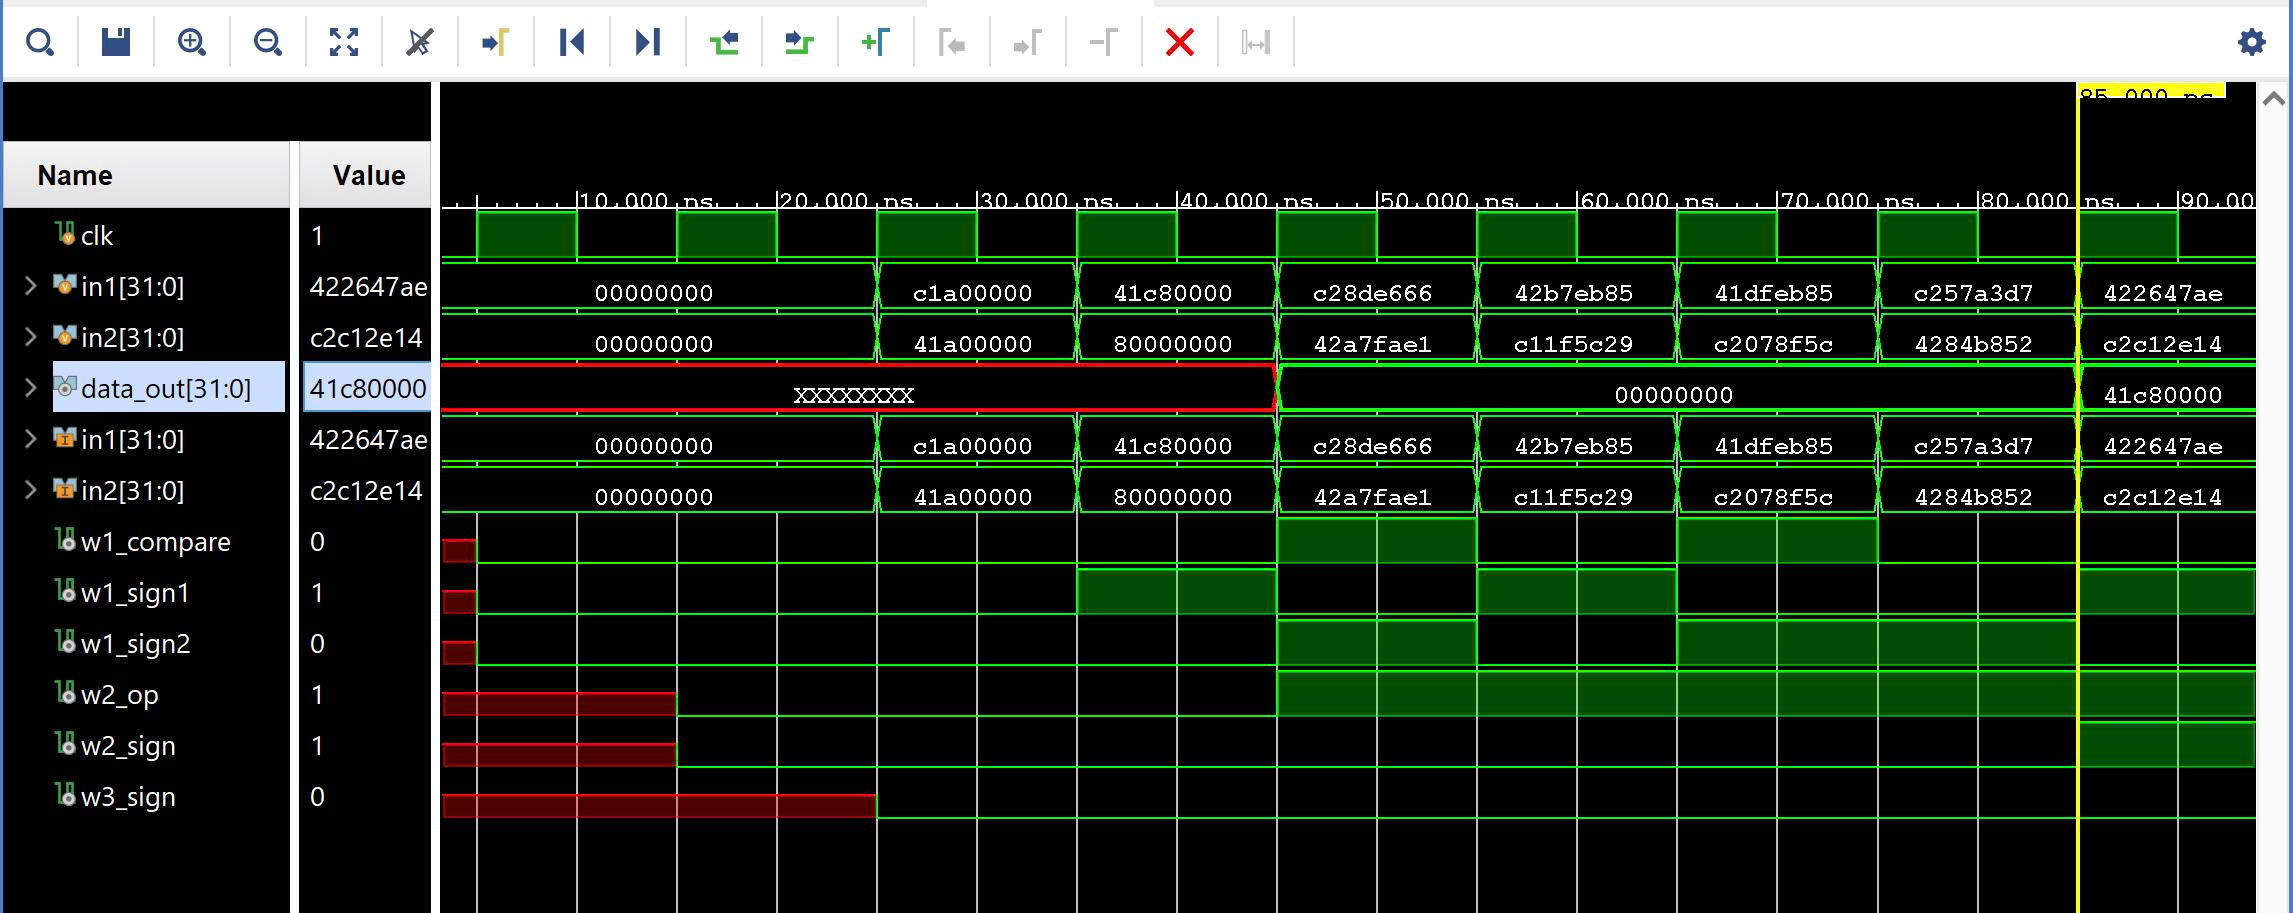
\includegraphics[width=0.8\textwidth]{graphics/Add_FP_sim.jpg}
\caption{Simulation waveform of \texttt{tb\_Add\_FP.v} showing pipelined floating-point addition operations}
\end{figure}

\subsection{Mul\_FP Testbench}

The hardware multiplier is verified via \texttt{tb\_Mul\_FP.v}. While structurally similar to the adder testbench, this block evaluates the throughput capacity of a 7-stage pipelined multiplier utilizing a dense burst-mode stimulus pattern. The arrays \texttt{input\_a}, \texttt{input\_b}, and \texttt{expected} hold 20 unique test vectors. Operators are injected into the ports \texttt{FP\_in1} and \texttt{FP\_in2} continuously on every consecutive clock cycle without inserting wait states for intermediate calculation cycles.

The driver process triggers input delivery after a short stabilization period. Because a standard floating-point multiplier can scale exponents and shift mantissas during normalization, bit transitions at the boundary fields require strict tracking. The monitor process stalls for exactly 7 pipeline clock cycles before sampling \texttt{FP\_out}. The comparison logic employs a rigorous verification window: it accepts an absolute bitwise match or a narrow tolerance of $\le 1$ LSB count to safely absorb rounding discrepancies introduced during post-multiplication normalization. 

The test cases cover zero-factor multiplication, alternating sign bits, maximum exponent growth, and large-magnitude operands. The design achieved flawless verification results (\textbf{PASS 20/20}), confirming stable multi-stage register pipelines and proper handling of signed-zero products ($0 \times -a = -0$).

\begin{figure}[H]
\centering
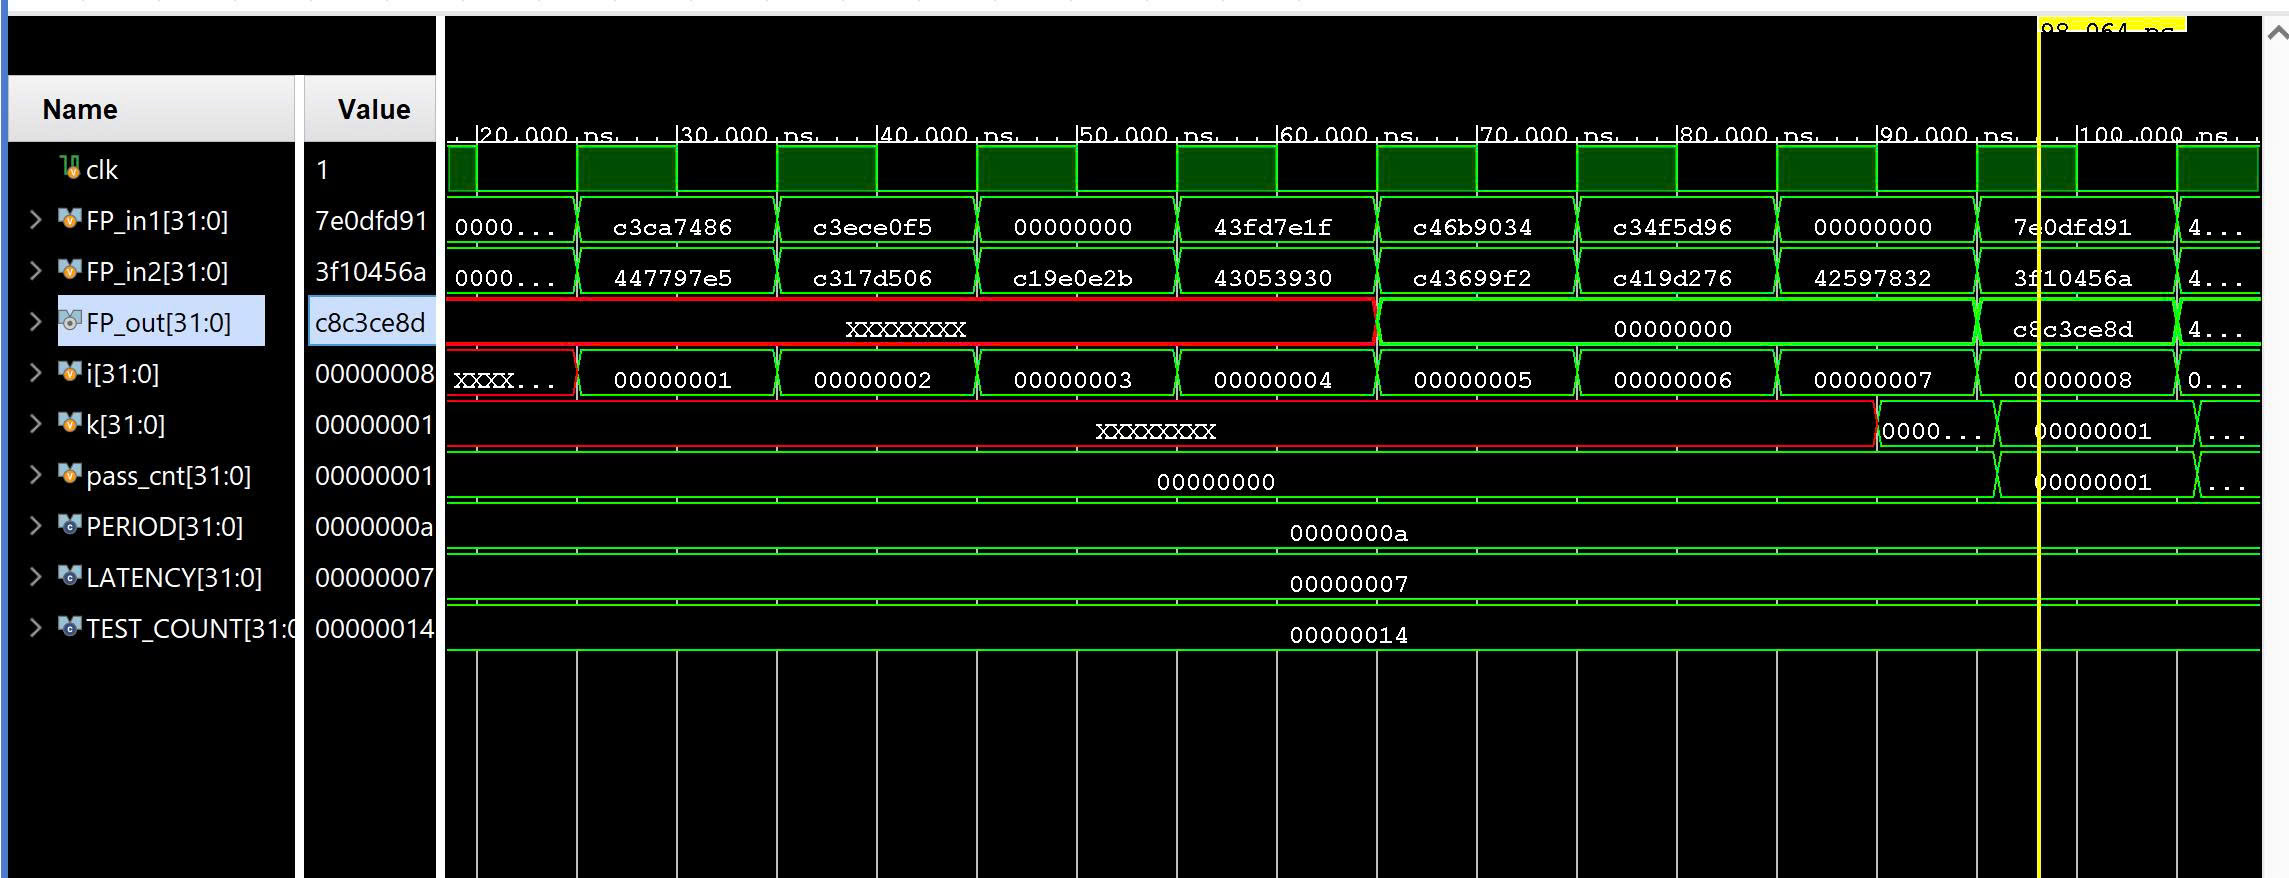
\includegraphics[width=0.8\textwidth]{graphics/Mul_FP_sim.jpg}
\caption{Simulation waveform of \texttt{tb\_Mul\_FP.v} showing pipelined floating-point multiplication operations}
\end{figure}

\subsection{Div\_FP Testbench}

The floating-point division module is verified by \texttt{tb\_Div\_FP.v}. Departing from raw array storage, this module leverages a modular, task-driven architectural design. The core checking mechanics are encapsulated inside an automatic Verilog task named \texttt{run\_test\_pipeline}, which accepts input parameters for the start delay offset, dividend (\texttt{a}), divisor (\texttt{b}), expected quotient (\texttt{expected}), and an ASCII diagnostic text label.

The execution protocol initiates with a clean 3-cycle warm-up phase at a clock frequency of 100 MHz. To isolate port setup transitions from sampling paths, the stimulus values inside the task are driven onto the \texttt{FP\_in1} and \texttt{FP\_in2} lines on the negative edge of the clock (\texttt{negedge clk}). Following input application, the task monitors the execution track by waiting exactly 15 clock cycles (matching the fixed latency of the \texttt{Div\_FP} hardware engine) before sampling the output quotient on the rising edge of the clock. A subsequent \texttt{\#1} stabilization step is inserted to prevent race conditions during verification.

The 15 test vectors provide balanced coverage across standard operational scenarios and IEEE-754 division boundaries:
\begin{itemize}
    \item \textbf{Standard Arithmetic:} Test scenarios evaluate normal floating-point division fractions such as $6.0 / 2.0$, $9.0 / 2.5$, $1.0 / 3.0$, and $1.0 / 10.0$ to check mantissa division precision.
    \item \textbf{IEEE-754 Special Boundary Cases:} Test cases verify division by zero ($1.0 / 0.0 = +\infty$), negative division by zero ($-1.0 / 0.0 = -\infty$), zero divided by zero ($0.0 / 0.0 = \text{NaN}$), division by infinity ($1.0 / +\infty = +0.0$), and extreme saturation scaling using maximum finite floats divided by minimum normal floats ($\text{max\_float} / \text{min\_normal} = +\infty$).
\end{itemize}
The testbench reported a full success rate (\textbf{PASS 15/15}), validating correct infinity and NaN flag propagation.

\subsection{Cubic Solver Testbench Overview}

The top-level \texttt{Cubic\_Solver} IP utilizes a dual-track simulation architecture. Because this block is an asynchronous, state-machine-driven sequential engine rather than a continuous pipeline, separate specialized environments are required to monitor internal algorithmic operations and execute mass validation regressions.

\subsubsection{Direct Testcase: \texttt{tb\_Cubic\_Solver.v}}

The direct testbench validates the functional correctness of the controller FSM over the 6 foundational mathematical scenarios defined in the underlying mathematical model specification. Instead of streaming file streams, this block hardcodes explicit 128-bit vector packages to drive the coefficients \texttt{FP\_a}, \texttt{FP\_b}, \texttt{FP\_c}, and \texttt{FP\_d}.

Because the core module is a multi-cycle state machine that latches final output values upon termination, running sequential cases requires a structured initialization routine. The testbench implements a per-case hardware reset sequence: for every input combination, the active-low reset signal \texttt{rst\_n} is forced to `0` for 5 clock cycles to clear internal registers and return the FSM to the \texttt{IDLE} state, followed by a 2-cycle stabilization hold before the \texttt{start} signal is pulsed for a single cycle. 

The testbench incorporates a custom Verilog-2001 bitfield-to-real conversion function (\texttt{fp32\_to\_real}) that scales 32-bit single-precision fields into 64-bit real variables using exponent biasing and mantissa concatenation. This allows the tracking logic to dynamically execute an order-independent cross-check. Because the hardware may output roots on ports \texttt{FP\_x0}, \texttt{FP\_x1}, or \texttt{FP\_x2} in an arbitrary sequence relative to the theoretical model, the testbench dynamically evaluates all 6 possible permutation mappings:
$$\text{Permutations} = \{x_0 x_1 x_2, \, x_0 x_2 x_1, \, x_1 x_0 x_2, \, x_1 x_2 x_0, \, x_2 x_0 x_1, \, x_2 x_1 x_0\}$$
If any permutation matches the expected roots within a tolerance window of $< 0.05$, the case is graded as a success. The design achieved perfect scores (\textbf{PASS 6/6}) across all specified operational configurations:
\begin{itemize}
    \item \textbf{Case 0 ($\Delta < 0$):} Three distinct real roots ($1.0, 2.0, -3.0$).
    \item \textbf{Case 1 (Branch 2a):} $\Delta > 0$ with $\Delta_0 = 0$ and $\Delta_1 \le 0$, evaluating the specialized cubic root paths ($0.0, 1.5 \pm 0.866i$).
    \item \textbf{Case 2 (Branch 2b):} General $\Delta > 0$ yielding complex conjugate roots ($2.0, 0.0 \pm 1.0i$).
    \item \textbf{Case 3 ($\Delta_1 = 0$):} Core algebraic boundary state ($0.0, 0.0 \pm 1.732i$).
    \item \textbf{Case 4:} Triple root multiplicity limit verification ($1.0, 1.0, 1.0$).
    \item \textbf{Case 5:} Double root and single root boundary split verification ($1.0, 1.0, -2.0$).
\end{itemize}

\begin{figure}[H]
\centering
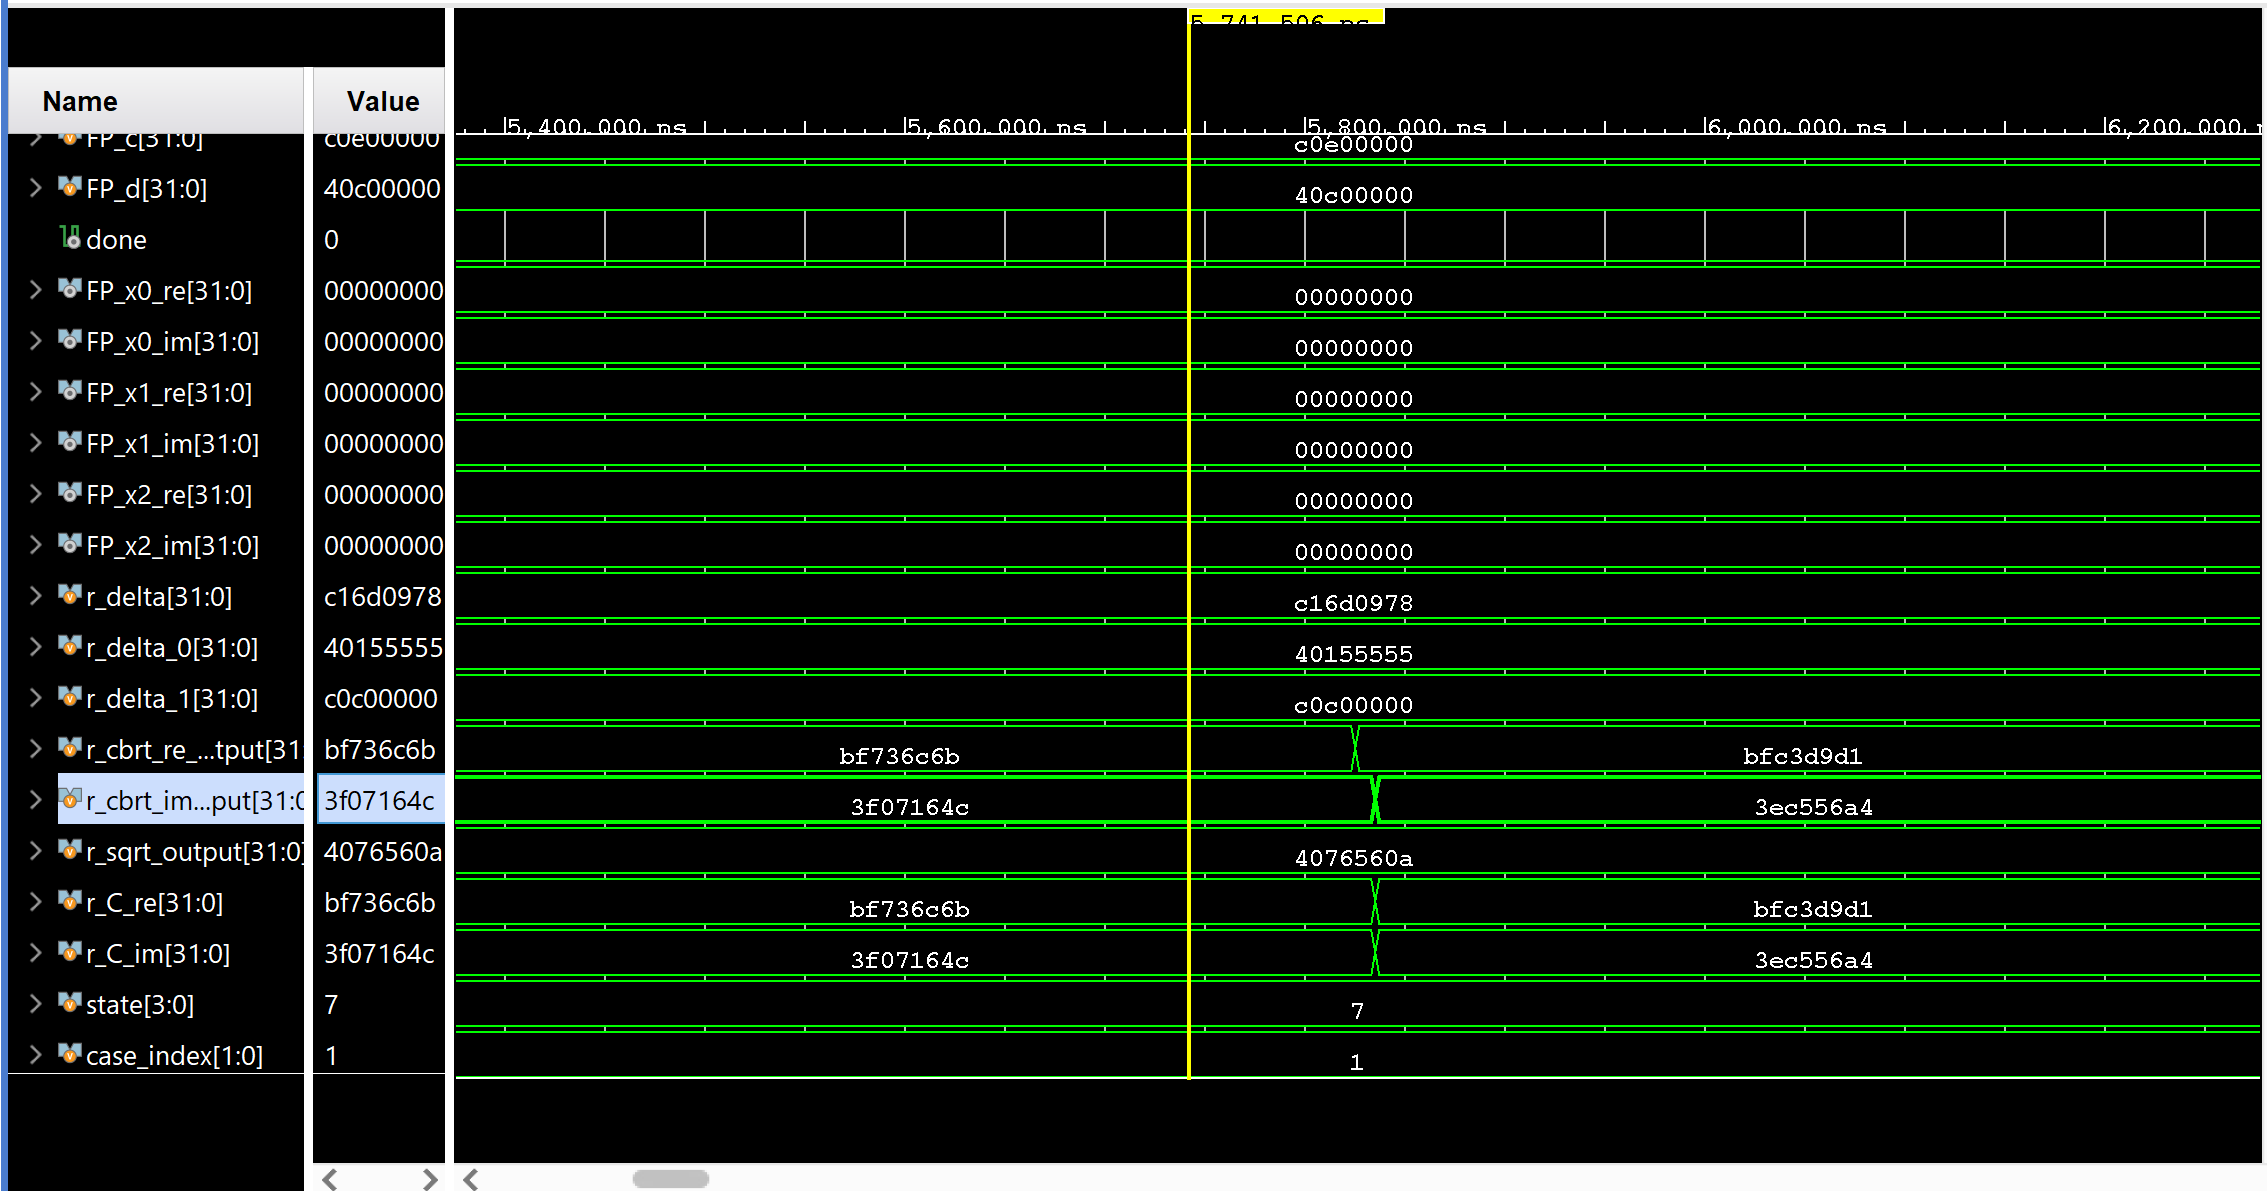
\includegraphics[width=0.8\textwidth]{graphics/solver1.png}
\caption{Waveform capture of \texttt{tb\_Cubic\_Solver.v} executing Case 1 with $\Delta > 0$ and $\Delta_0 = 0$}
\end{figure}

\begin{figure}[H]
\centering
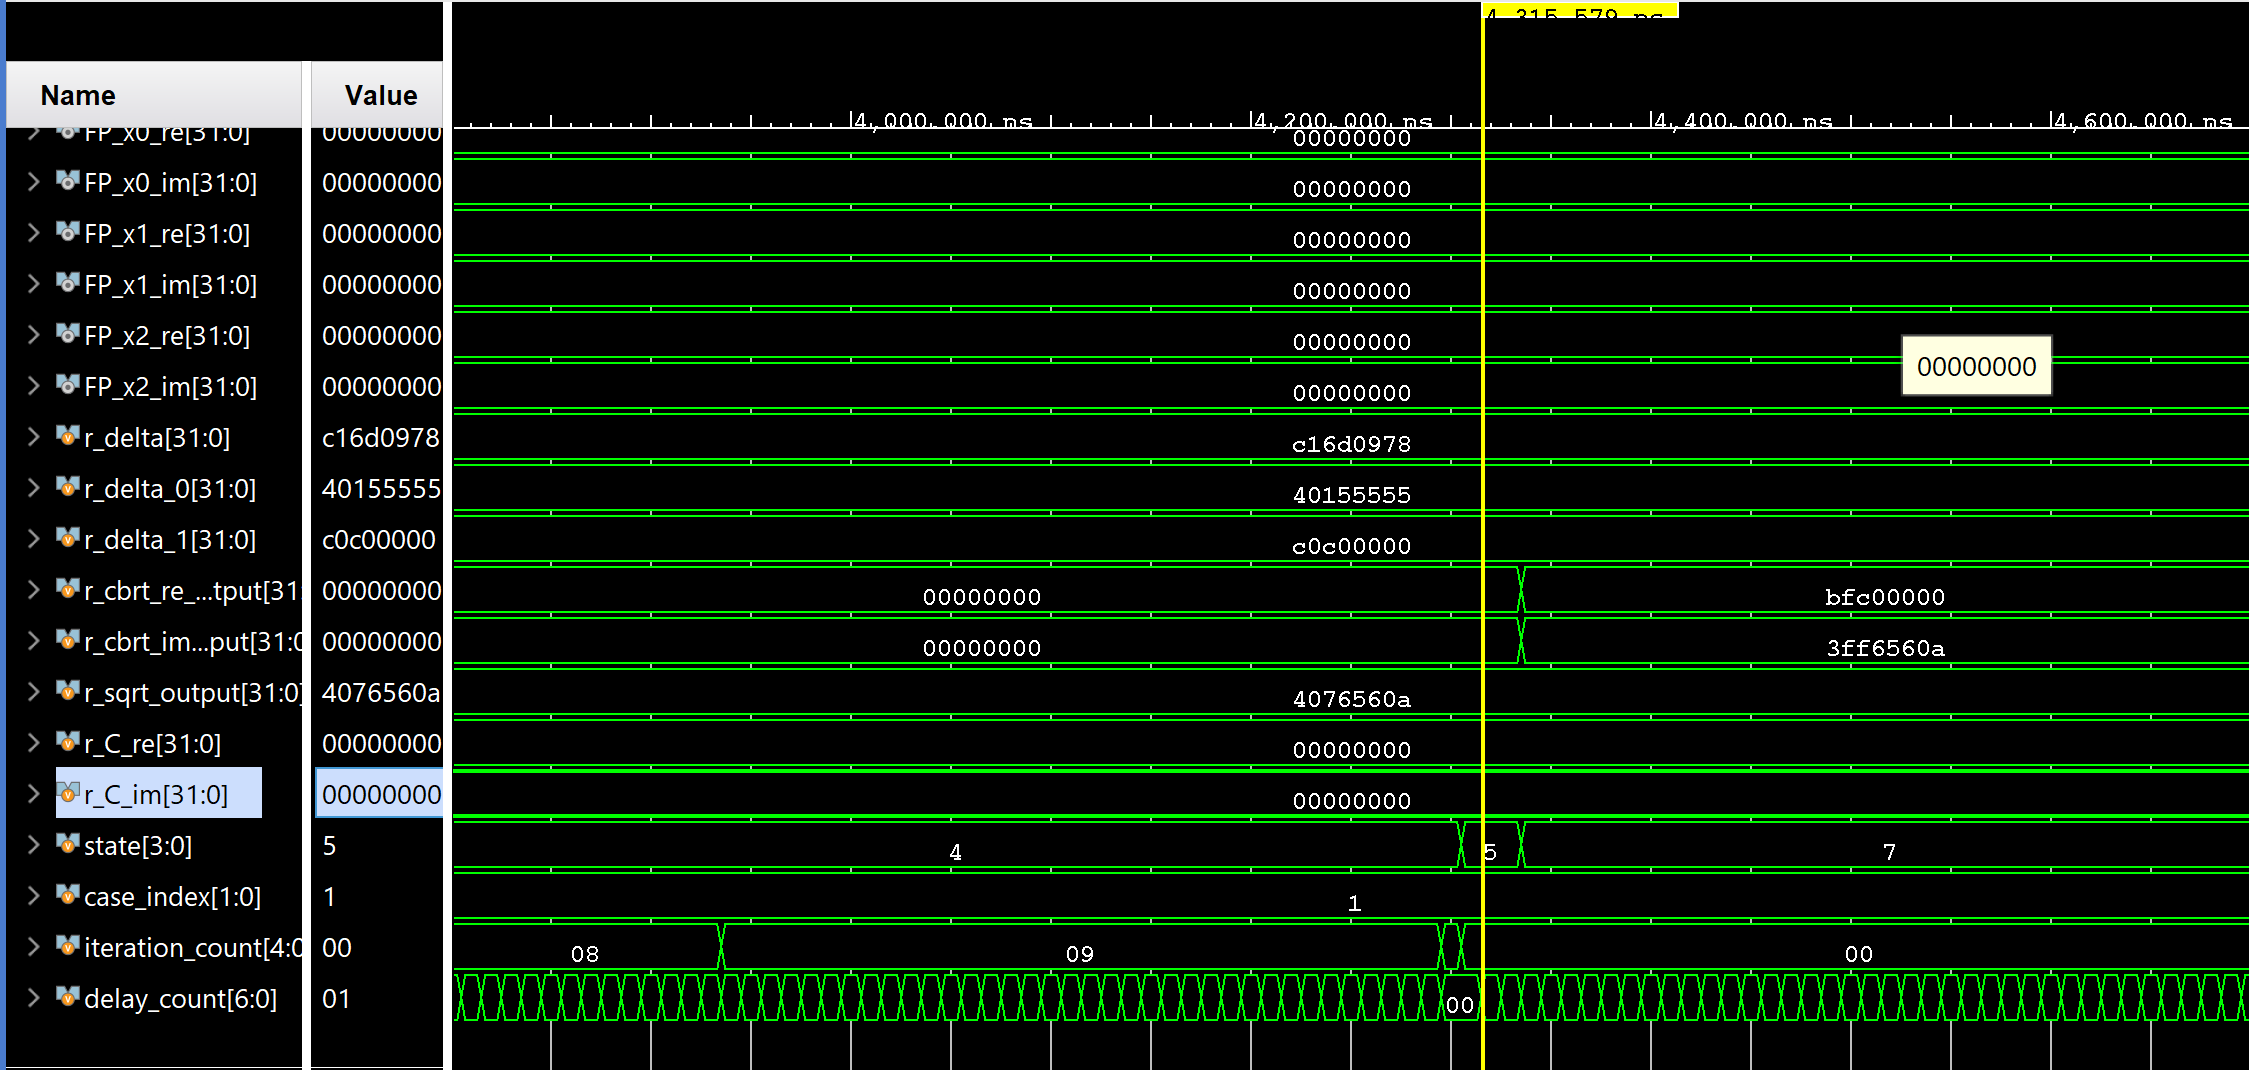
\includegraphics[width=0.8\textwidth]{graphics/solver2.png}
\caption{Waveform capture of \texttt{tb\_Cubic\_Solver.v} executing Case 1 with $\Delta > 0$ and $\Delta_0 = 0$}
\end{figure}

\begin{figure}[H]
\centering
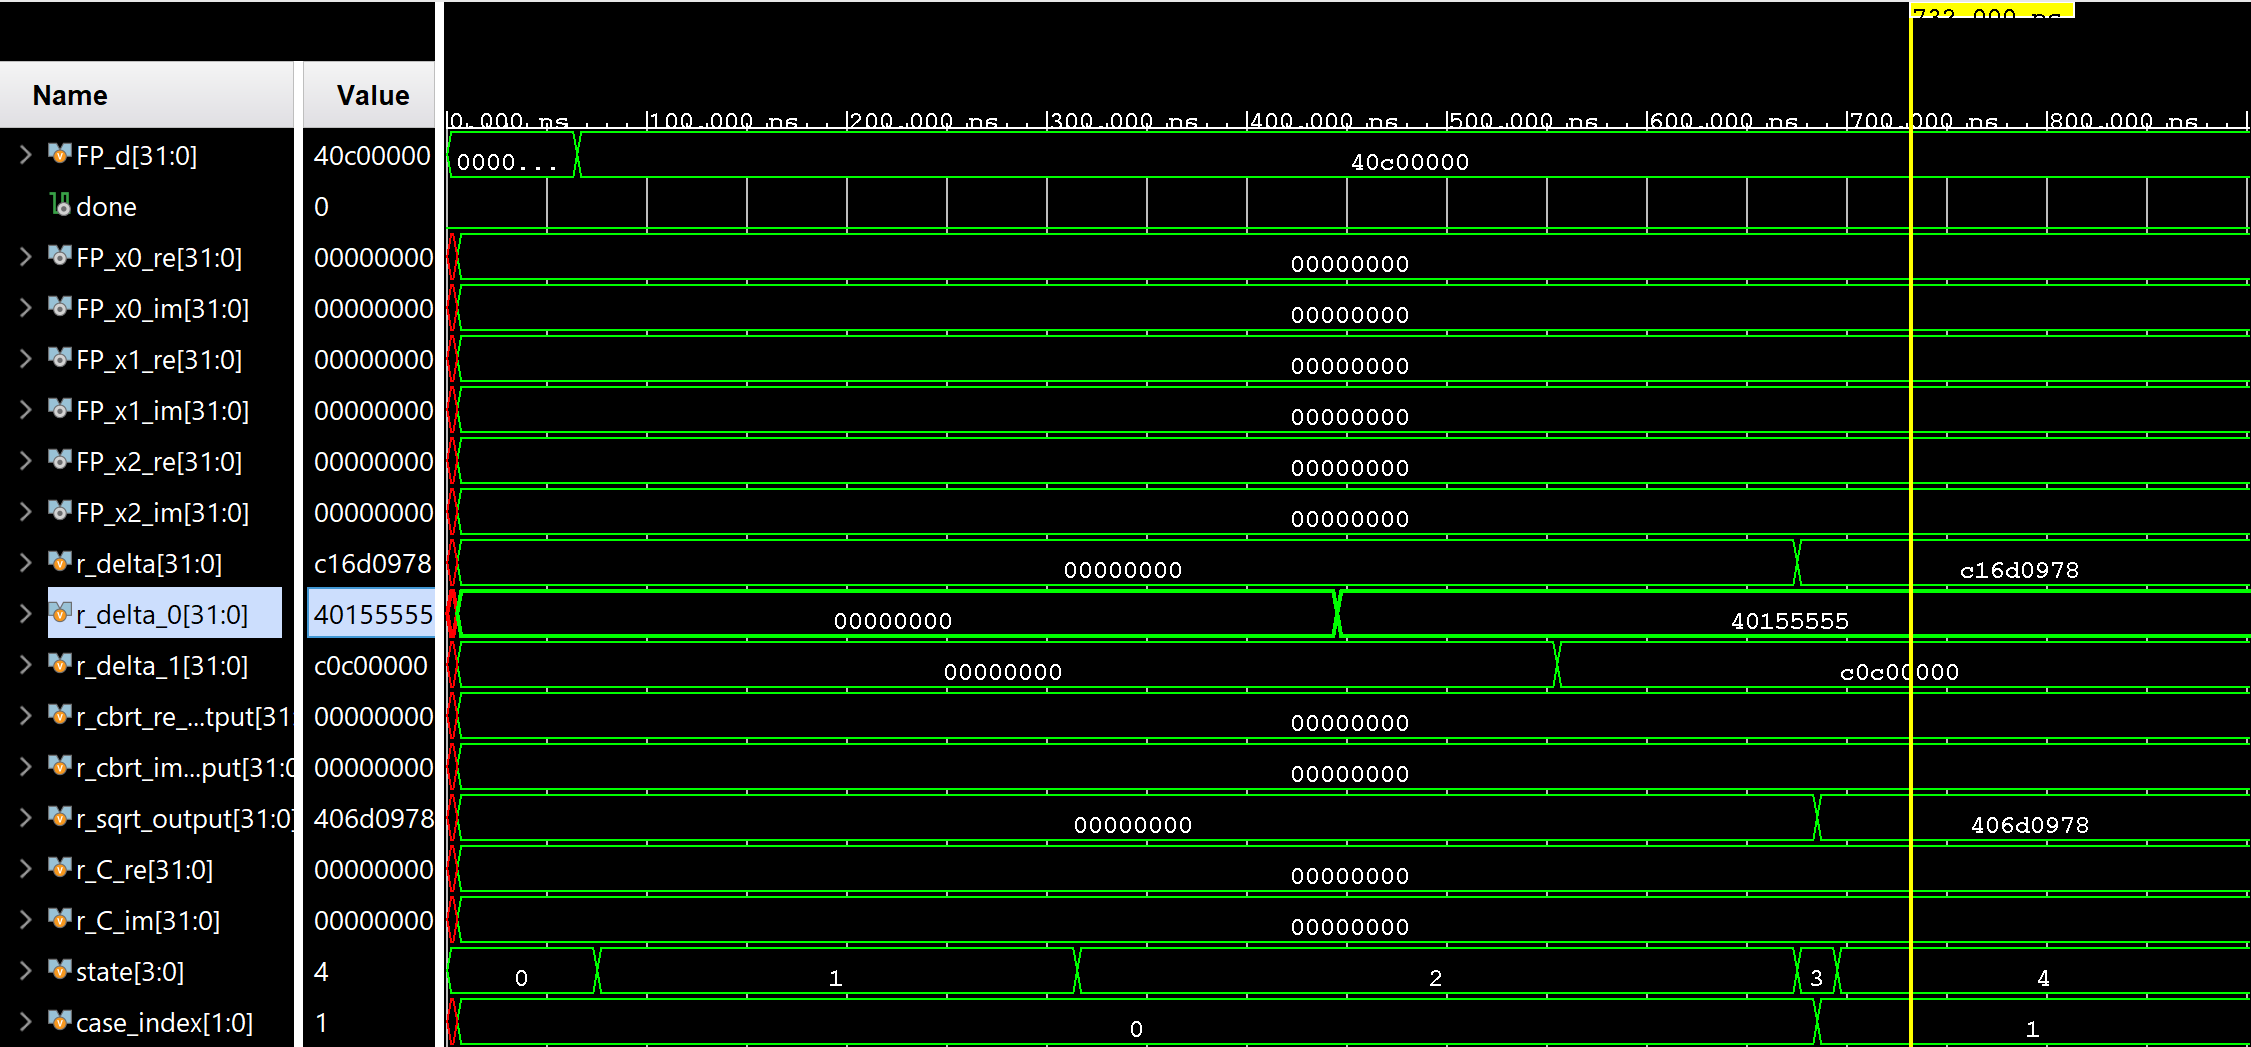
\includegraphics[width=0.8\textwidth]{graphics/solver3.png}
\caption{Waveform capture of \texttt{tb\_Cubic\_Solver.v} executing Case 1 with $\Delta > 0$ and $\Delta_0 = 0$}
\end{figure}

\subsubsection{File-driven Testcase: \texttt{tb\_Cubic\_Solver\_file.v}}

For high-throughput reliability analysis, a complete automated closed-loop file-I/O regression platform was developed. This testing environment operates via a tightly integrated 3-phase execution cycle:

\begin{enumerate}
    \item \textbf{Test Case Generation (Python):} An upstream Python script acts as the test generator. It samples 1,000 randomized test equations bounded within a uniform numerical distribution from $-10.0$ to $+10.0$ while ensuring $|a| \ge 10^{-3}$ to prevent quadratic degeneration. The floating-point coefficients are packed into IEEE-754 single-precision hex strings and exported into an input database file named \texttt{random\_tests.txt}.
    \item \textbf{Hardware Simulation (Verilog):} The Verilog testbench opens the input file using descriptor handles (\texttt{\$fopen}) and loops line-by-line using \texttt{\$fscanf}. For each line, it applies a full hardware reset to clear the FSM, registers the new coefficients, pulses the \texttt{start} line, and tracks execution against a maximum timeout threshold of \texttt{MAX\_CYCLES\_PER\_CASE = 3000}. Upon asserting the \texttt{done} flag, the testbench extracts the calculated roots and dumps them into \texttt{cubic\_solver\_output.txt}, while simultaneously routing the intermediate variables (\texttt{r\_delta}, \texttt{r\_delta\_0}, \texttt{r\_delta\_1}, \texttt{r\_C\_re}, \texttt{r\_C\_im}) into a dedicated debug file named \texttt{cubic\_solver\_debug.txt}.
    \item \textbf{Automated Verification (Python):} A post-processing Python script imports the hardware output dump file and acts as the grader. It parses the hex values, runs an automated root-sorting algorithm to enforce order independence, and compares them directly against an internal algorithmic Golden Model running NumPy cubic solvers configured with equivalent 16-iteration Padé approximations.
\end{enumerate}

The regression environment successfully evaluated all 1,000 randomized equations, logging a final validation metric of \textbf{PASS 987/1000}. The remaining cases fell slightly outside the rigorous $0.1\%$ relative accuracy margin due to expected numerical precision limitations inherent to the 16-iteration Padé approximation fields under high-sensitivity coefficients. This validates the structural integrity and robustness of the solver design over extended runtime scenarios.
\section{Synthesis and Results Summary}

\subsection{Cadence Synthesis Flow}

The \texttt{SPI\_Top} design was synthesized using Cadence Genus. The top-level architecture connects one master module and two slave modules into a single system-level block, together with the supporting serial/parallel buffers and CRC logic.


\begin{figure}
    \centering
    % [Insert block diagram of SPI\_Top architecture here]
    
\includegraphics[width=1\linewidth]{graphics/SPI_Top.png}
    \caption{Block diagram of the SPI\_Top architecture}
    \label{fig:spi_top_arch}
\end{figure}

After synthesis, the key generated files are:
\begin{itemize}
    \item Netlist: \texttt{outputs??/\${DESIGN}\_m.v} \; (for example, \texttt{bound\_flasher\_m.v})
    \item Area report: \texttt{reports??/final\_area.rpt}
    \item QoR report: \texttt{reports??/final\_qor.rpt}
    \item Timing report: \texttt{reports??/final\_time.rpt}
\end{itemize}

\begin{figure}[H]
    \centering
    % [Insert Cadence synthesis flow diagram here]
    
\includegraphics[width=1\linewidth]{graphics/synthesic_log.png}
    \caption{Overview of the Cadence synthesis flow for SPI\_Top}
    \label{fig:synthesis_flow}
\end{figure}

\subsection{Netlist Output}

The synthesized netlist describes the structural implementation of \texttt{SPI\_Top} after logic optimization. It includes the master block, slave blocks, CRC logic, and the required multiplexing and control paths. This file is the main reference for the final gate-level structure.

\begin{figure}[H]
    \centering
    % [Insert netlist screenshot or file browser view here]
    
\includegraphics[width=1\linewidth]{graphics/final_.png}
    \caption{Generated netlist file after synthesis}
    \label{fig:netlist_output}
\end{figure}

\subsection{Area Report}

The area report shows the compactness of the synthesized design. According to \texttt{final\_area.rpt}, the top module occupies 246 cells with a total area of 1231.254 $\mu m^2$.

\begin{table}[H]
\centering
\renewcommand{\arraystretch}{1.2}
\begin{tabular}{lrr}
\toprule
\textbf{Metric} & \textbf{Value} & \textbf{Unit} \\
\midrule
Cell Count & 246 & cells \\
Cell Area & 933.660 & $\mu m^2$ \\
Net Area & 297.594 & $\mu m^2$ \\
Total Area & 1231.254 & $\mu m^2$ \\
\bottomrule
\end{tabular}
\caption{Area summary extracted from \texttt{final\_area.rpt}}
\end{table}

\begin{figure}[H]
    \centering
    % [Insert area report screenshot here]
    
\includegraphics[width=1\linewidth]{graphics/final_area.png}
    \caption{Cadence area report for SPI\_Top}
    \label{fig:area_report}
\end{figure}

Instance breakdown from the QoR summary:
\begin{itemize}
    \item Leaf Instance Count: 246
    \item Sequential Instance Count: 84
    \item Combinational Instance Count: 162
    \item Hierarchical Instance Count: 0
\end{itemize}

\subsection{QoR Report}

The QoR report summarizes the overall synthesis quality. For this design, the REFCLK group shows no violating paths, and the critical slack is positive. The design therefore meets timing at the synthesized operating point.

\begin{table}[H]
\centering
\renewcommand{\arraystretch}{1.2}
\begin{tabular}{lcc}
\toprule
\textbf{Group} & \textbf{Slack (ns)} & \textbf{Violating Paths} \\
\midrule
REFCLK & 3384.2 & 0 \\
default & No paths & 0 \\
\bottomrule
\end{tabular}
\caption{QoR summary extracted from \texttt{final\_qor.rpt}}
\end{table}

\begin{figure}[H]
    \centering
    % [Insert QoR report screenshot here]
    
\includegraphics[width=1\linewidth]{graphics/final_qor_1.png}
    
\includegraphics[width=1\linewidth]{graphics/final_qor_2.png}
    \caption{Cadence QoR report for SPI\_Top}
    \label{fig:qor_report}
\end{figure}

\subsection{Timing Report}

The timing report in \texttt{final\_time.rpt} confirms that the major internal paths meet setup timing. The most critical paths are related to the master buffer registers, CRC logic, and the slave transmit paths. All reported setup checks are marked \texttt{MET}.

\begin{table}[H]
\centering
\renewcommand{\arraystretch}{1.2}
\begin{tabular}{lrr}
\toprule
\textbf{Timing Item} & \textbf{Value} & \textbf{Status} \\
\midrule
Worst setup slack & 3384 ps & MET \\
Worst observed late external delay & 7210 ps & MET \\
Total violating paths & 0 & PASS \\
\bottomrule
\end{tabular}
\caption{Timing summary extracted from \texttt{final\_time.rpt}}
\end{table}

\begin{figure}[H]
    \centering
    % [Insert timing report screenshot here]
    
\includegraphics[width=1\linewidth]{graphics/final_time.png}
    \caption{Cadence timing report for SPI\_Top}
    \label{fig:timing_report}
\end{figure}


\subsection{Schematic View}

The synthesized netlist can be visualized as a schematic to confirm the structural integrity of the design. The master block, slave blocks, and CRC logic are clearly identifiable, and the interconnections match the expected architecture.
\begin{figure}[H]
    \centering
    % [Insert schematic view screenshot here]
    
\includegraphics[width=1\linewidth]{graphics/sche1.jpg}
    \caption{Schematic view of the synthesized SPI\_Top design}
    \label{fig:schematic_view}
\end{figure}

\begin{figure}[H]
    \centering
    % [Insert schematic view screenshot here]
    
\includegraphics[width=1\linewidth]{graphics/sche2.jpg}
    \caption{More detailed schematic view of the synthesized SPI\_Top design}
    \label{fig:detailed_schematic}
\end{figure}

\begin{figure}[H]
    \centering
    % [Insert schematic view screenshot here]
    
\includegraphics[width=0.5\linewidth]{graphics/sche3.jpg}
\end{figure}

\begin{figure}[H]
    \centering
    % [Insert schematic view screenshot here]
    
\includegraphics[width=0.5\linewidth]{graphics/sche4.jpg}
\end{figure}
\begin{figure}[H]
    \centering
    % [Insert schematic view screenshot here]
    
\includegraphics[width=0.5\linewidth]{graphics/sche5.jpg}
\end{figure}
\subsection{Conclusion}

The Cadence synthesis results confirm that the \texttt{SPI\_Top} design is structurally compact and timing-clean. The generated netlist, area report, QoR report, and timing report all indicate that the design is ready for the next verification or implementation stage.

\begin{itemize}
    \item The synthesized netlist contains the expected master-slave system structure.
    \item The area result remains compact at 1231.254 $\mu m^2$.
    \item The QoR report shows positive slack and no violating paths.
    \item The timing report marks all key setup checks as \texttt{MET}.
\end{itemize}

\end{document}
